\documentclass[10pt,a4paper,titlepage]{article}
\usepackage[utf8]{inputenc}
\usepackage{amsmath}
\usepackage{amsfonts}
\usepackage{amssymb}
\usepackage{graphicx}
\usepackage{subcaption}
\usepackage{float}
\usepackage{tabularx}
%\usepackage{mwe}
\author{Claude Goubet}
\title{Project technical report 2: Split Bregman}
\begin{document}

\maketitle

\section{2D Split Bregman}
	
	\subsection{Scenarios description}
		\subsubsection{image samples}
		In order to reduce computation time for the comparison of scenarios and methods three sample images were selected. These sample are all 156*156 images representing relevant details that we wish to preserve from the full-size image.
		\begin{figure}[H]
		
       		\centering
      		\begin{subfigure}[b]{0.32\textwidth}
            	\centering
            	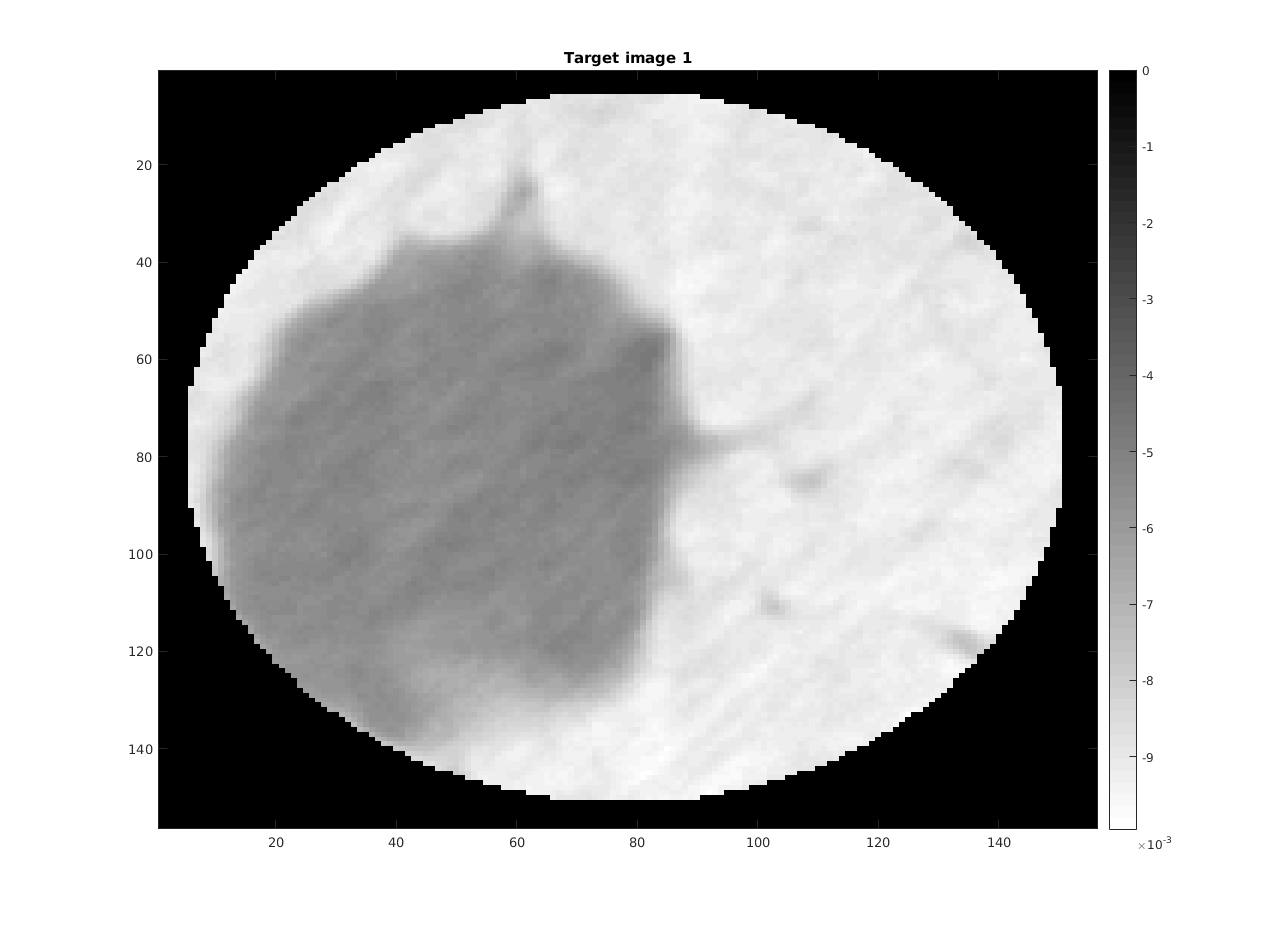
\includegraphics[width=\textwidth]{Sample1/target1.png}
            	\caption{Target 1}    
            	\label{subfig:Target1Fully}
        	\end{subfigure}
        	\hfill
        	\begin{subfigure}[b]{0.32\textwidth}  
            	\centering 
            	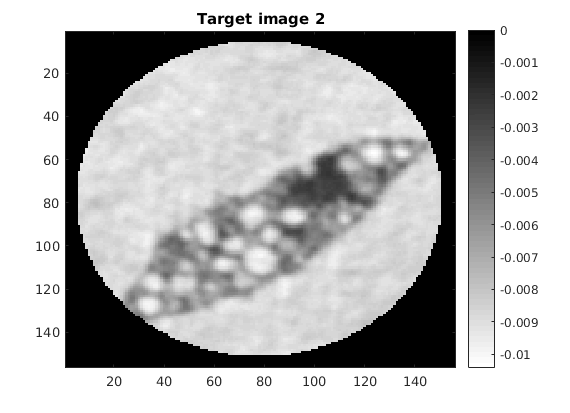
\includegraphics[width=\textwidth]{Sample2/target2.png}
            	\caption{Target 2}    
            	\label{subfig:FBP1Fully}
        	\end{subfigure}
        	\hfill
        	\begin{subfigure}[b]{0.32\textwidth}  
            	\centering 
            	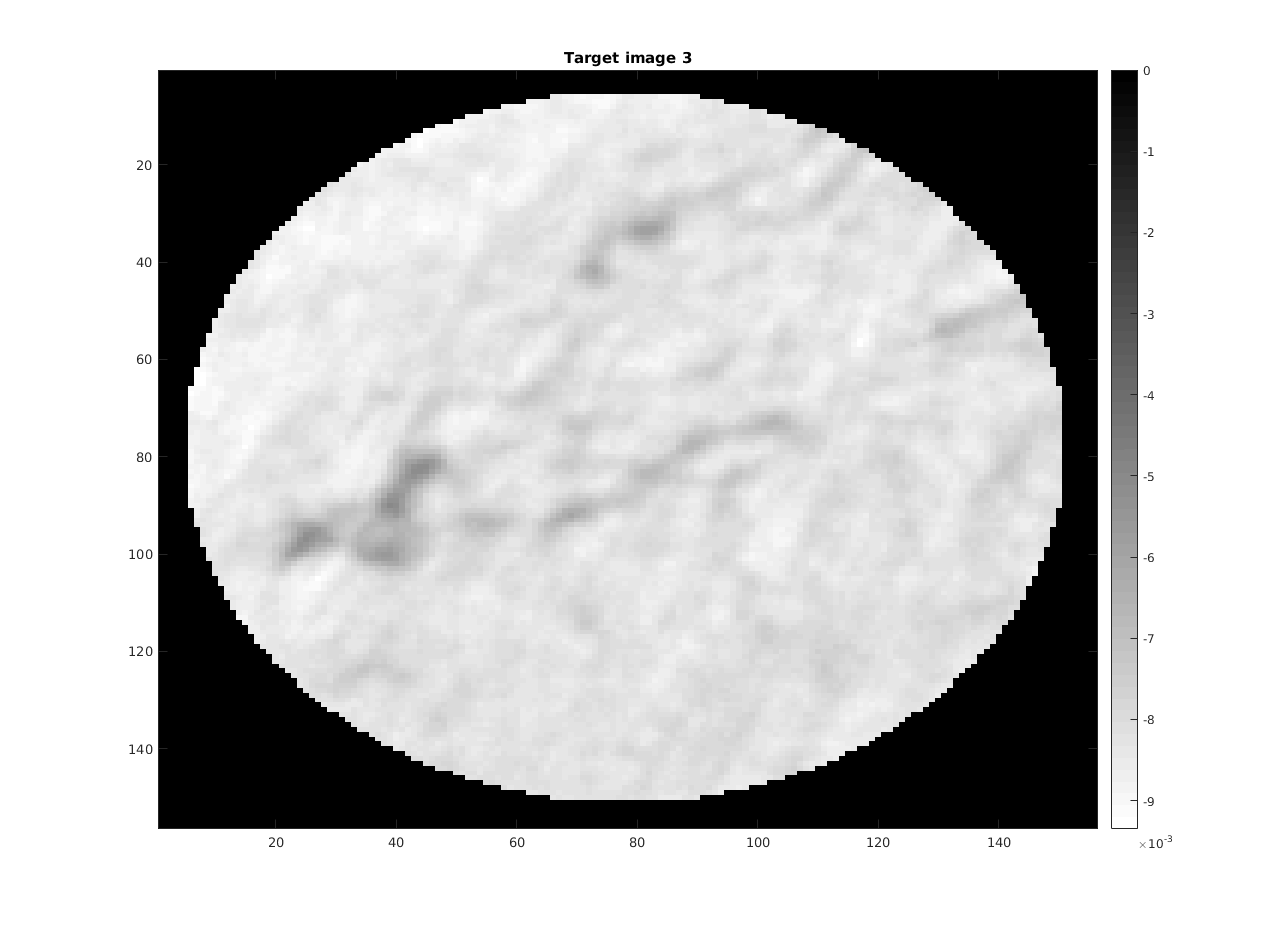
\includegraphics[width=\textwidth]{Sample3/target3.png}
            	\caption{Target 3}    
            	\label{subfig:FBP1Fully}
        	\end{subfigure}
        \end{figure}
		
		\subsubsection{scenarios}
			We defined multiple scenarios in order to test the algorithms. 
			\begin{itemize}
				\item We evaluate sequentially each target
				\item For each target we perform SB-TV on different number of iterations (20, 100, 200, 1000, 5000, 10000) (5000 and 10000 currently computing, I will change the code so that we save all these images in one call and not one call for each number of iterations)
				\item For each iteration number we perform SB-TV on different doses (100\%, 50\%, 25\% and 10\% of projection) (100\% projections being the image size).
			\end{itemize}					
			Future scenarios will be perform with noisy projections.
\clearpage

	\subsection{Image sample 1}
		\subsubsection{Fully projected (image size \#proj)}
			Use of 156 projections. We are here comparing the number of iterations of Split Bregman algorithm to the target and FBP images (respectively Figure \ref{subfig:Target1Fully} and \ref{subfig:FBP1Fully}. in Figure \ref{fig:retFully} are displayed 20, 200, 1000 and 5000 iterations.\\
			We can notice that the number of edges recovered increases with the number of iterations.\\
			In the next sections we will use 5000 iterations since it corresponds to the best image recovery.
			Some evaluation metrics are displayed in Table \ref{tab:Error2000Sample1}
		\begin{figure}[H]
		
       		\centering
      		\begin{subfigure}[b]{0.475\textwidth}
            	\centering
            	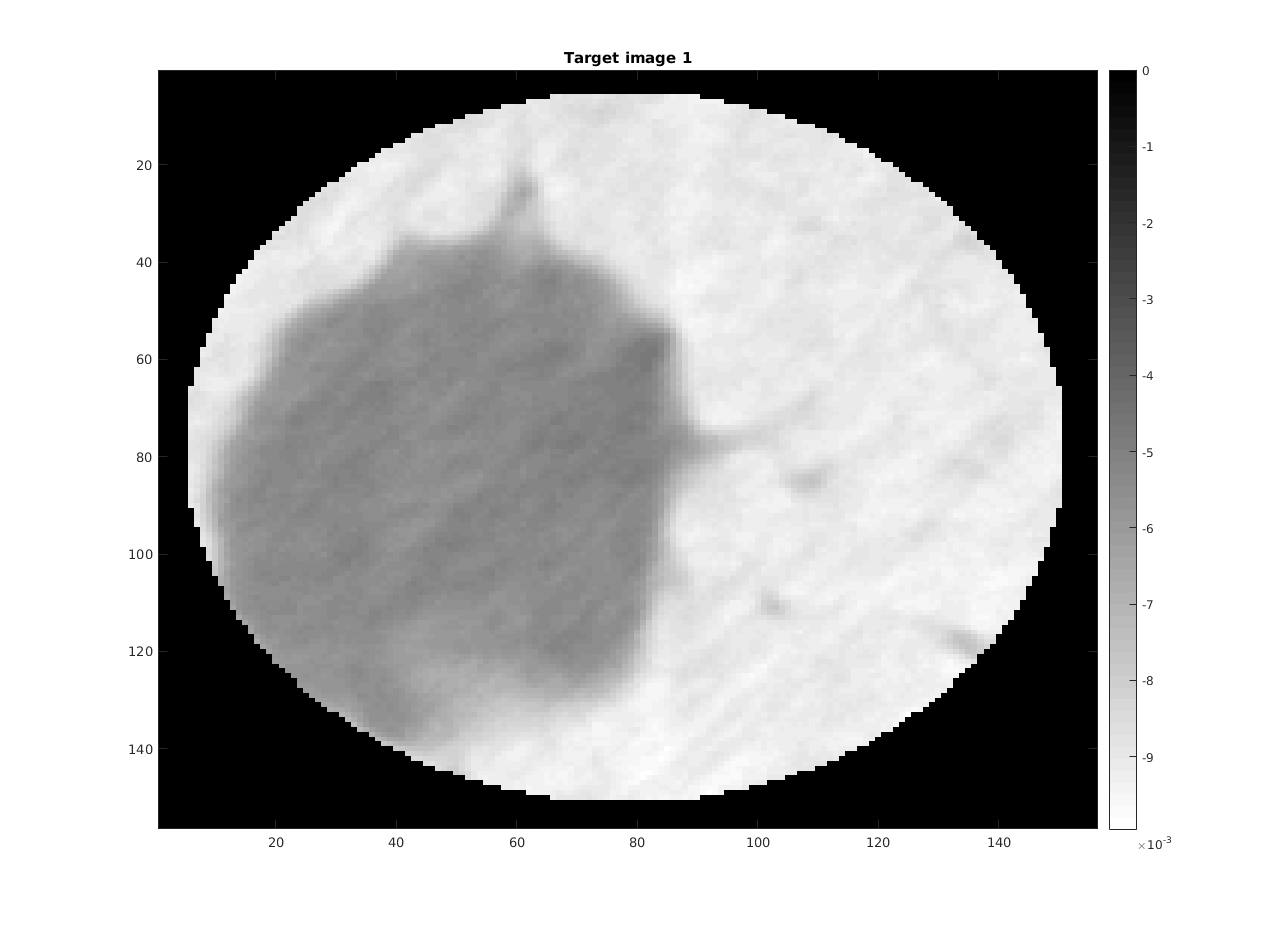
\includegraphics[width=\textwidth]{Sample1/target1.png}
            	\caption{Target image}    
            	\label{subfig:Target1Fully}
        	\end{subfigure}
        	\hfill
        	\begin{subfigure}[b]{0.475\textwidth}  
            	\centering 
            	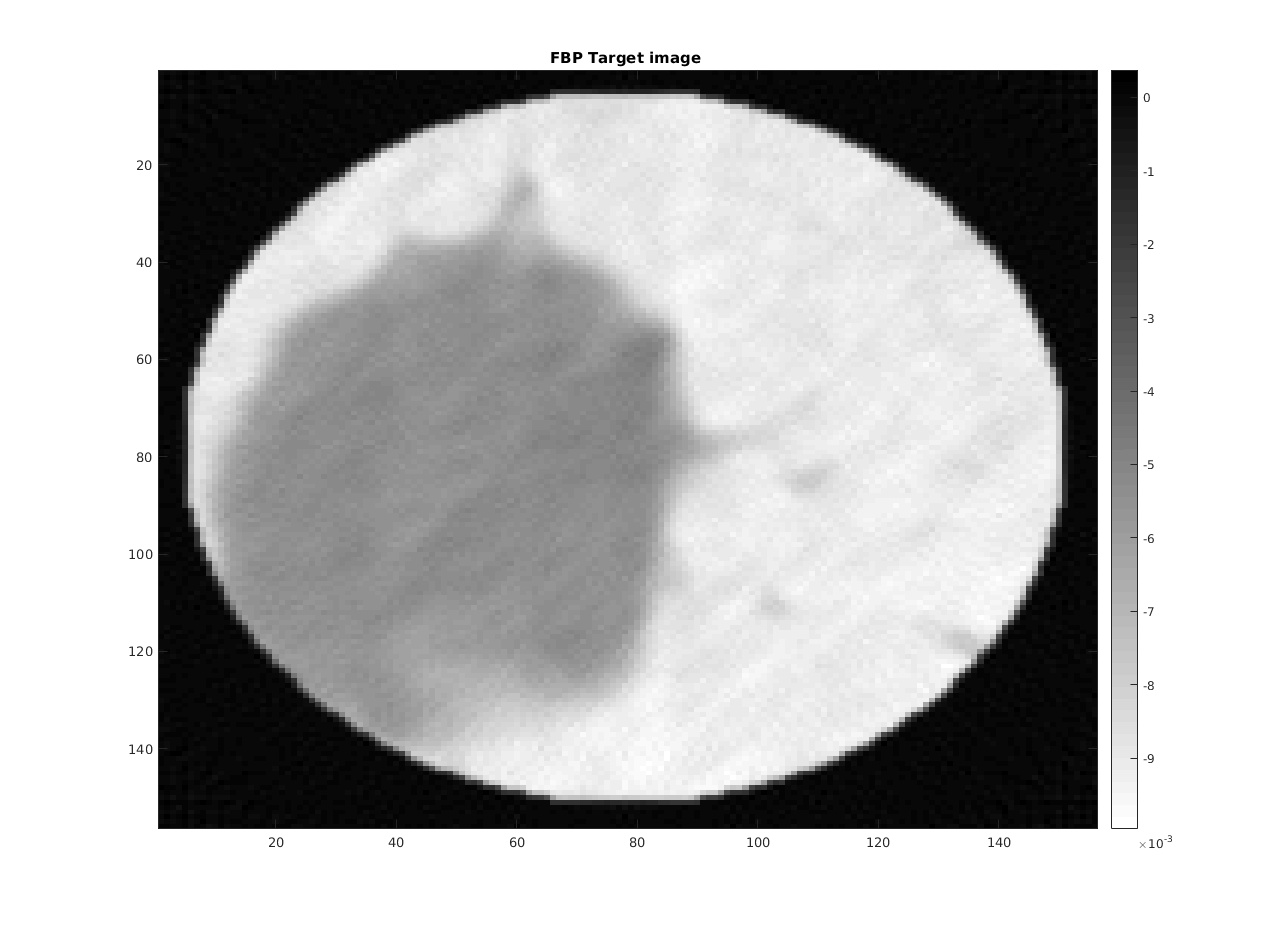
\includegraphics[width=\textwidth]{Sample1/fully/FBP.png}
            	\caption{FBP}    
            	\label{subfig:FBP1Fully}
        	\end{subfigure}
        	\vskip\baselineskip
        	\begin{subfigure}[b]{0.475\textwidth}   
        	    \centering 
            	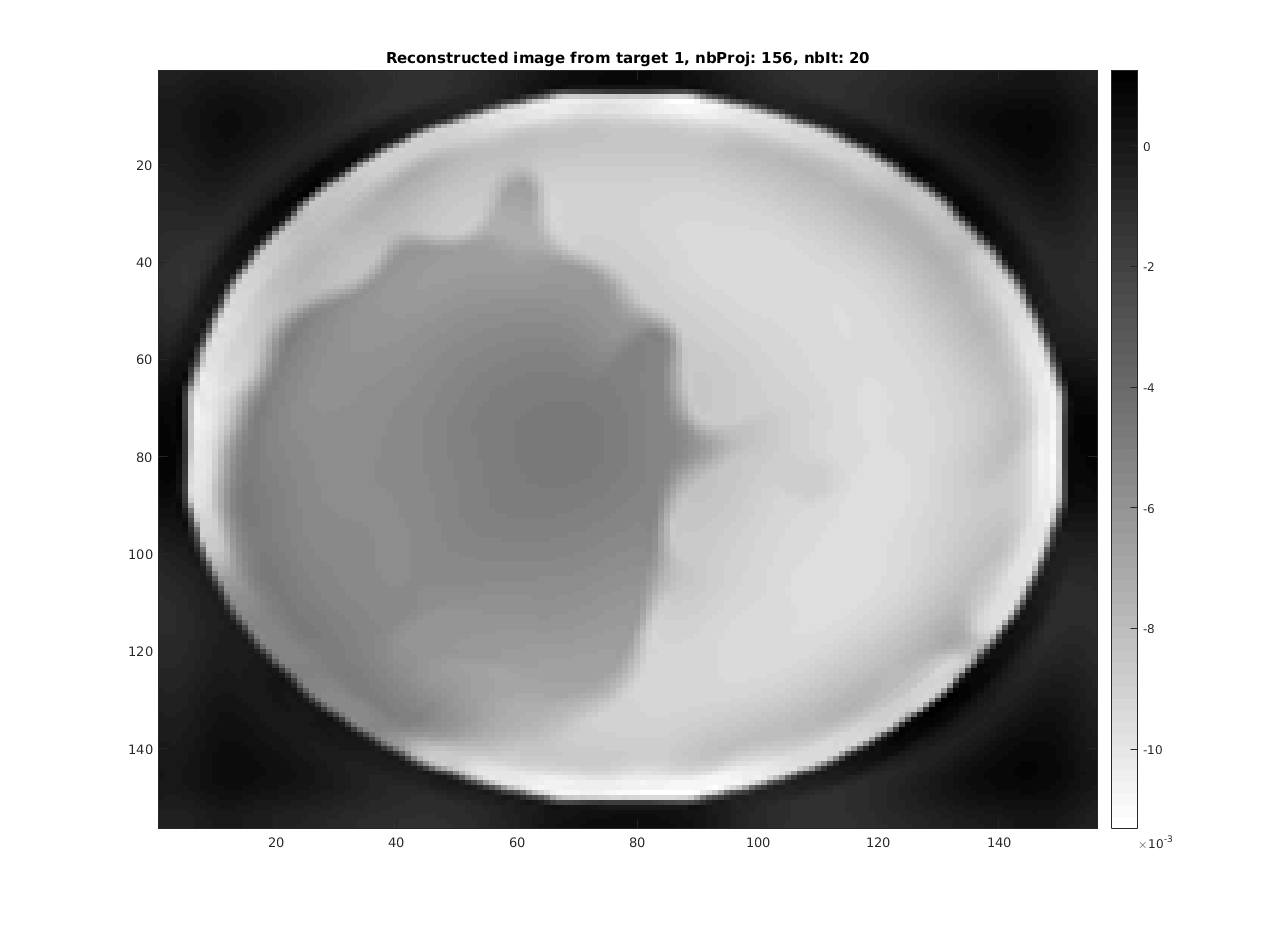
\includegraphics[width=\textwidth]{Sample1/fully/20it.png}
            	\caption{SB 20}  
            	\label{subfig:20it1Fully}
        	\end{subfigure}
        	\quad
        	\begin{subfigure}[b]{0.475\textwidth}   
        	    \centering 
        	    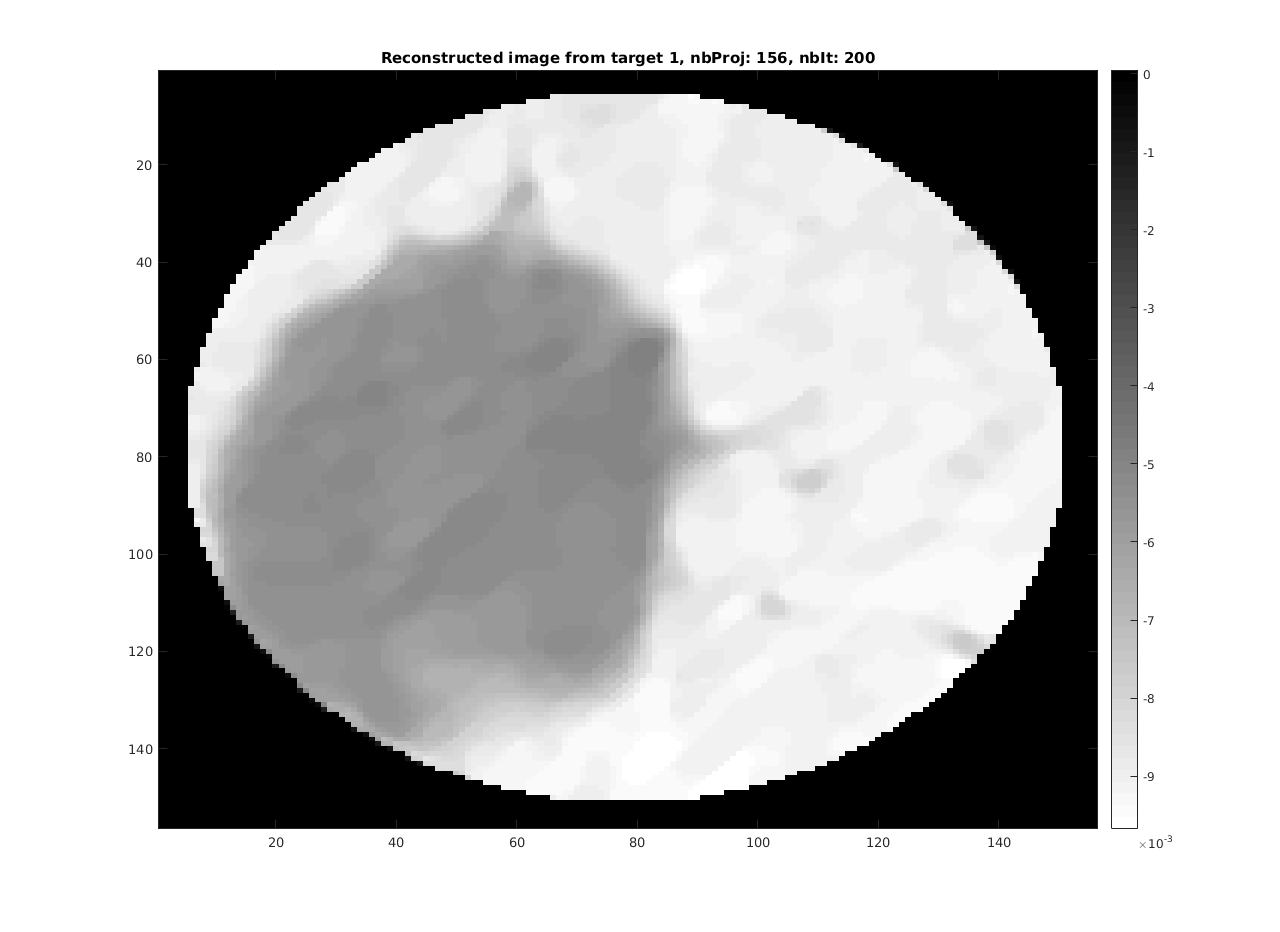
\includegraphics[width=\textwidth]{Sample1/fully/200it.png}
        	    \caption{SB 200}  
        	    \label{subfig:200it1Fully}
       		\end{subfigure}
        	\vskip\baselineskip
        	\begin{subfigure}[b]{0.475\textwidth}   
        	    \centering 
            	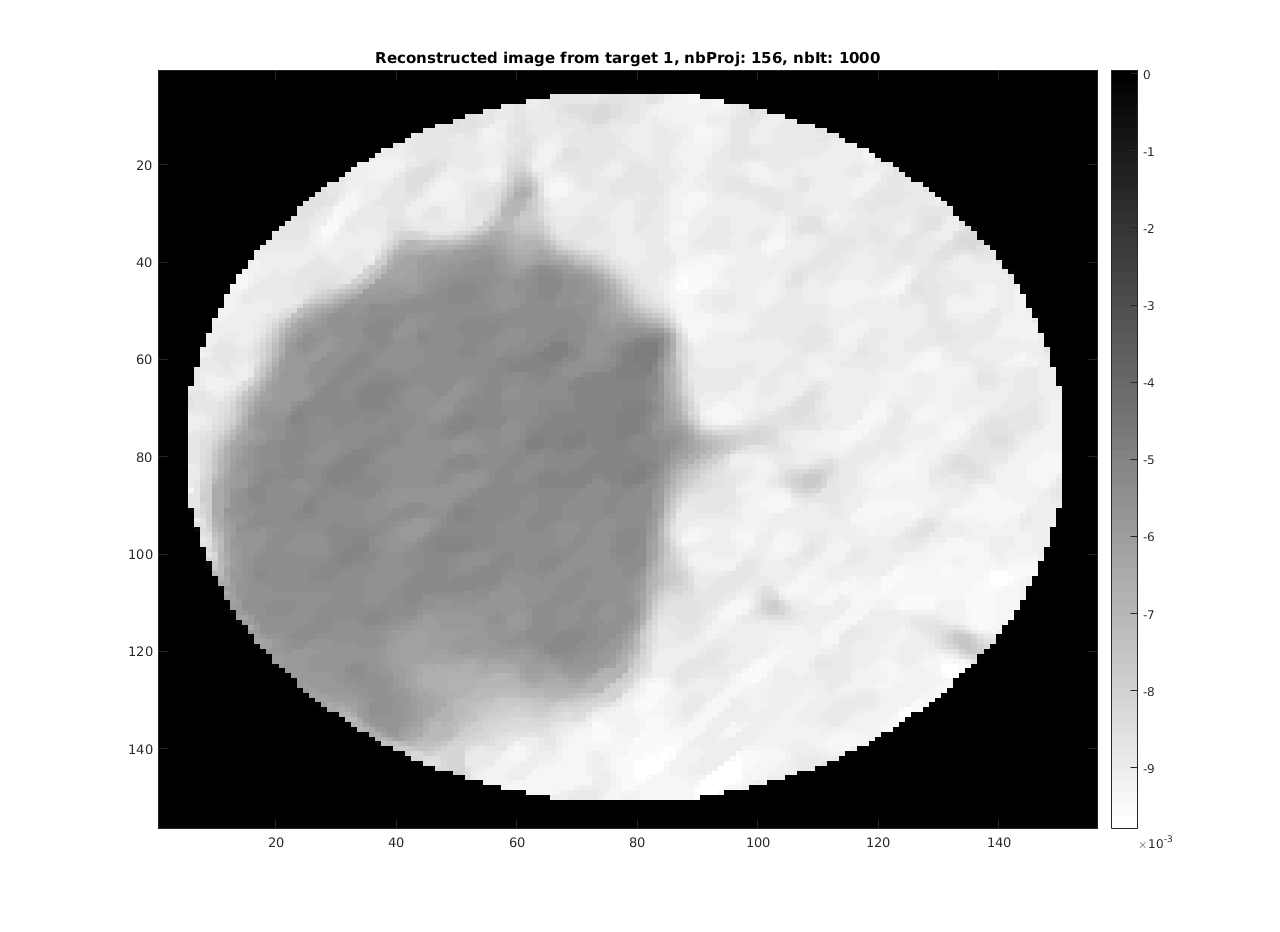
\includegraphics[width=\textwidth]{Sample1/fully/1000it.png}
            	\caption{SB 1000}
            	\label{subfig:1000it1Fully}
        	\end{subfigure}
        	\quad
        	\begin{subfigure}[b]{0.475\textwidth}   
        	    \centering 
        	    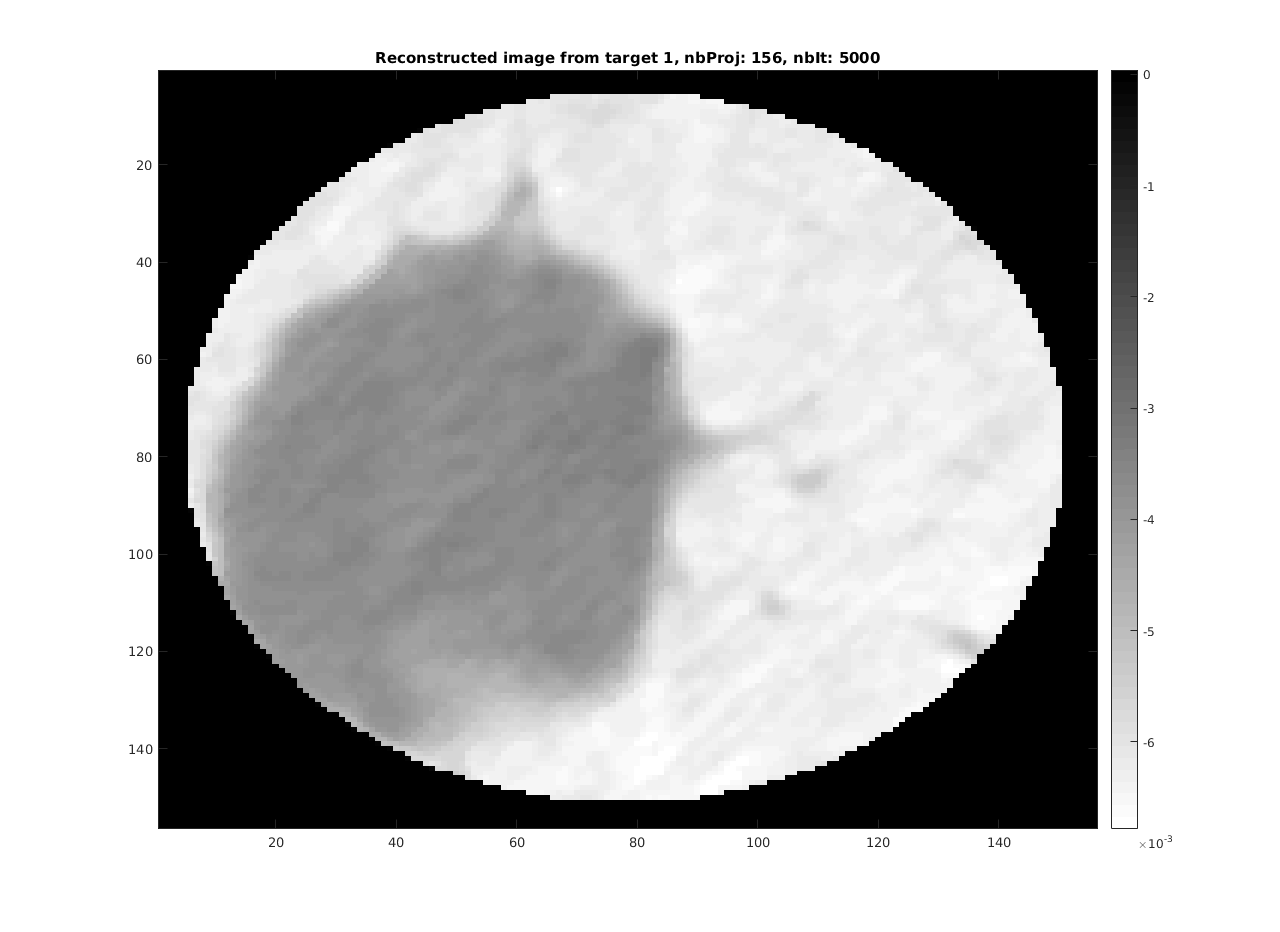
\includegraphics[width=\textwidth]{Sample1/fully/5000it.png}
        	    \caption{SB 5000}    
        	    \label{subfig:5000it1Fully}
       		\end{subfigure}
        	\caption{Retro-projections on fully projected object}
        	\label{fig:retFully}
    	\end{figure}

		\begin{table}[H]
			\begin{tabular}{ | l || c || c | c | c | c | r | }
 				\hline			
   				reconstruction	& FBP 	& SB 5000	& SB 1000	& SB 200	& SB 100	& SB 20 \\
   				\hline
  				Error			& 0.06	& 0.006		& 0.0081	& 0.0132	& 0.0244	& 0.1065 \\
 				\hline  
 				Time exec		&		& 11.96		& 62.45		& 129.66	& 647.87	& 3314	\\
 				\hline 
 			\end{tabular}
 			\caption{Reconstruction error rate from target image}
 			\label{tab:Error2000Sample1}
		\end{table}
\clearpage		
		\subsubsection{Sample 1 Low-Dose reconstruction}
		\textbf{reconstructed images}
		\begin{figure}[H]
		
       		\centering
      		\begin{subfigure}[b]{0.32\textwidth}
            	\centering
            	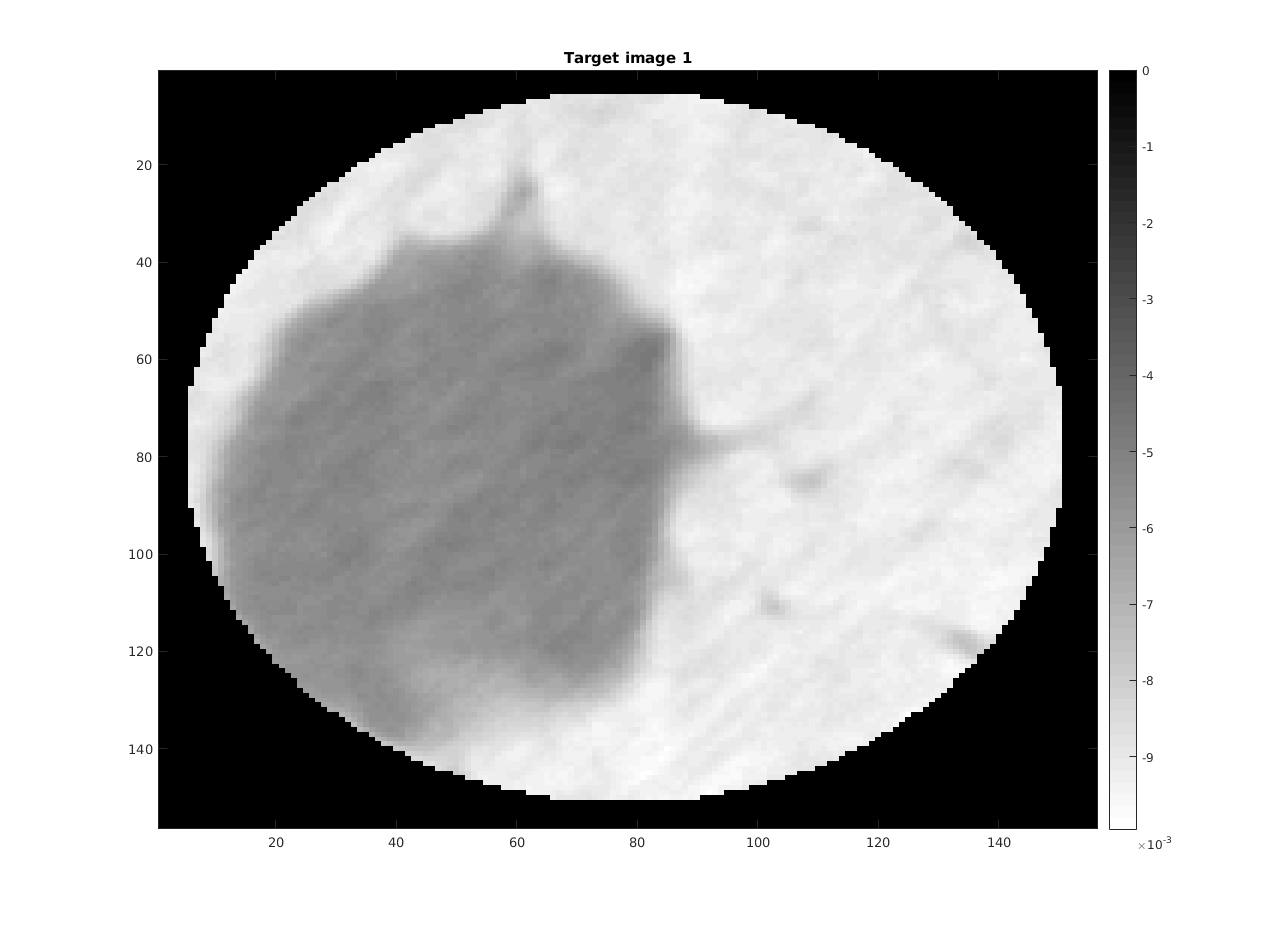
\includegraphics[width=\textwidth]{Sample1/target1.png}
            	\caption{Target image}    
            	%\label{subfig:Target1L-D}
        	\end{subfigure}
        	%\hfill
        	\begin{subfigure}[b]{0.32\textwidth}  
            	\centering 
            	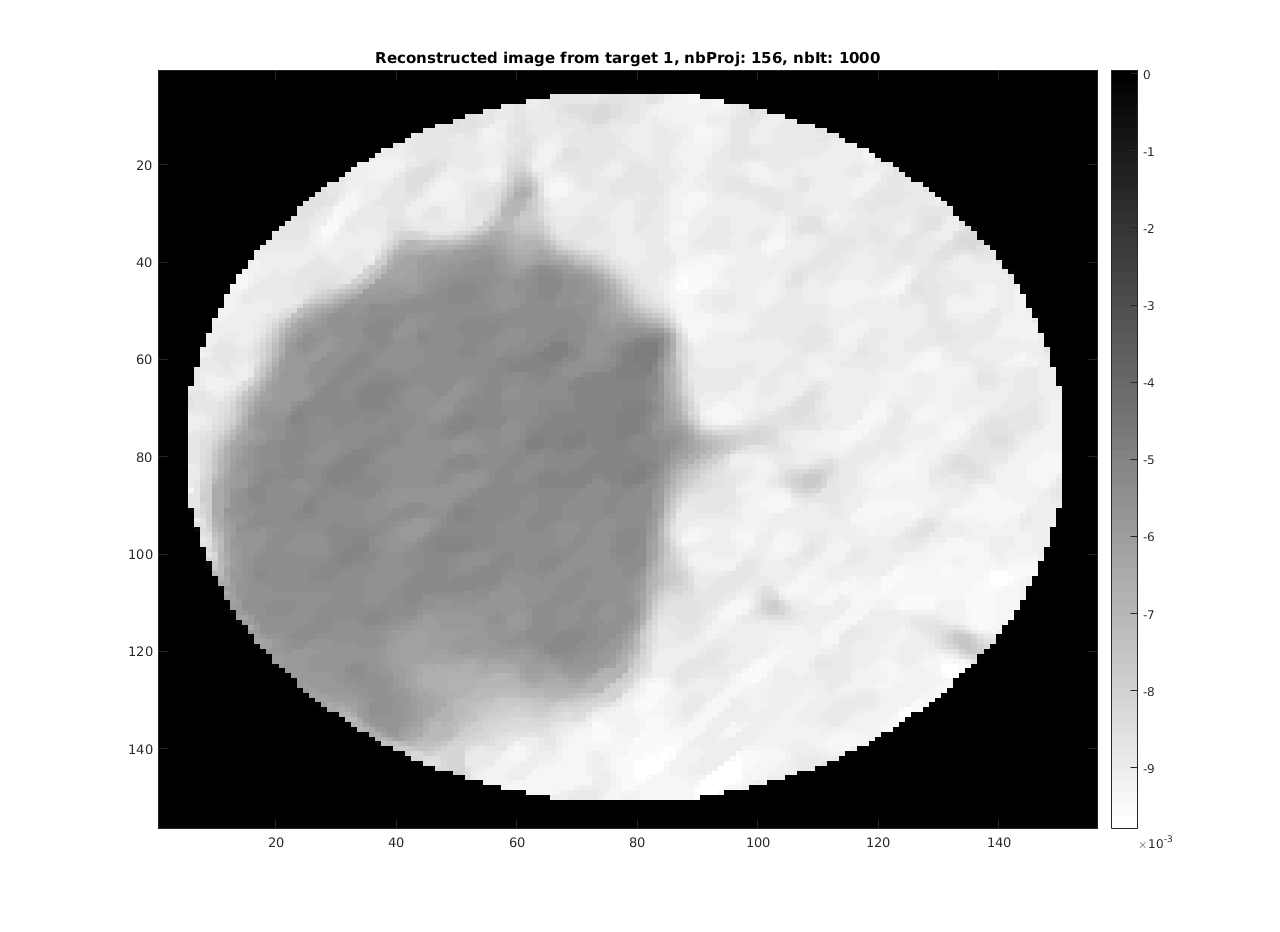
\includegraphics[width=\textwidth]{Sample1/L-D_5000/156p.png}
            	\caption{156 proj - 100\%}    
            	\label{subfig:156p1L-D}
        	\end{subfigure}
        	%\hfill
        	\begin{subfigure}[b]{0.32\textwidth}  
            	\centering 
            	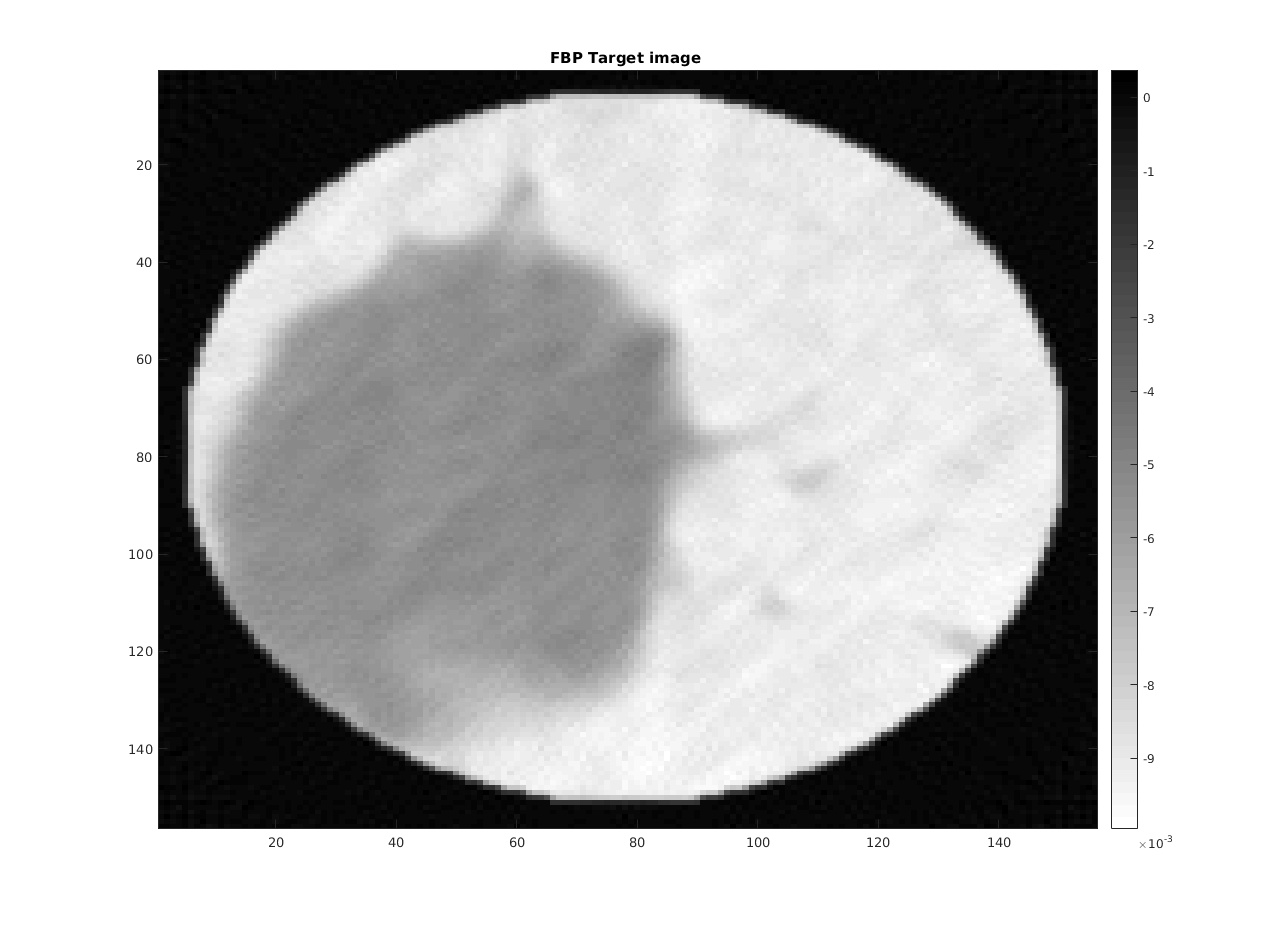
\includegraphics[width=\textwidth]{Sample1/L-D_5000/FBP156.png}
            	\caption{FBP}    
            	\label{subfig:FBP1156p}
        	\end{subfigure}
        	\vskip\baselineskip
        	
        	
        	\begin{subfigure}[b]{0.32\textwidth}   
        	    \centering 
            	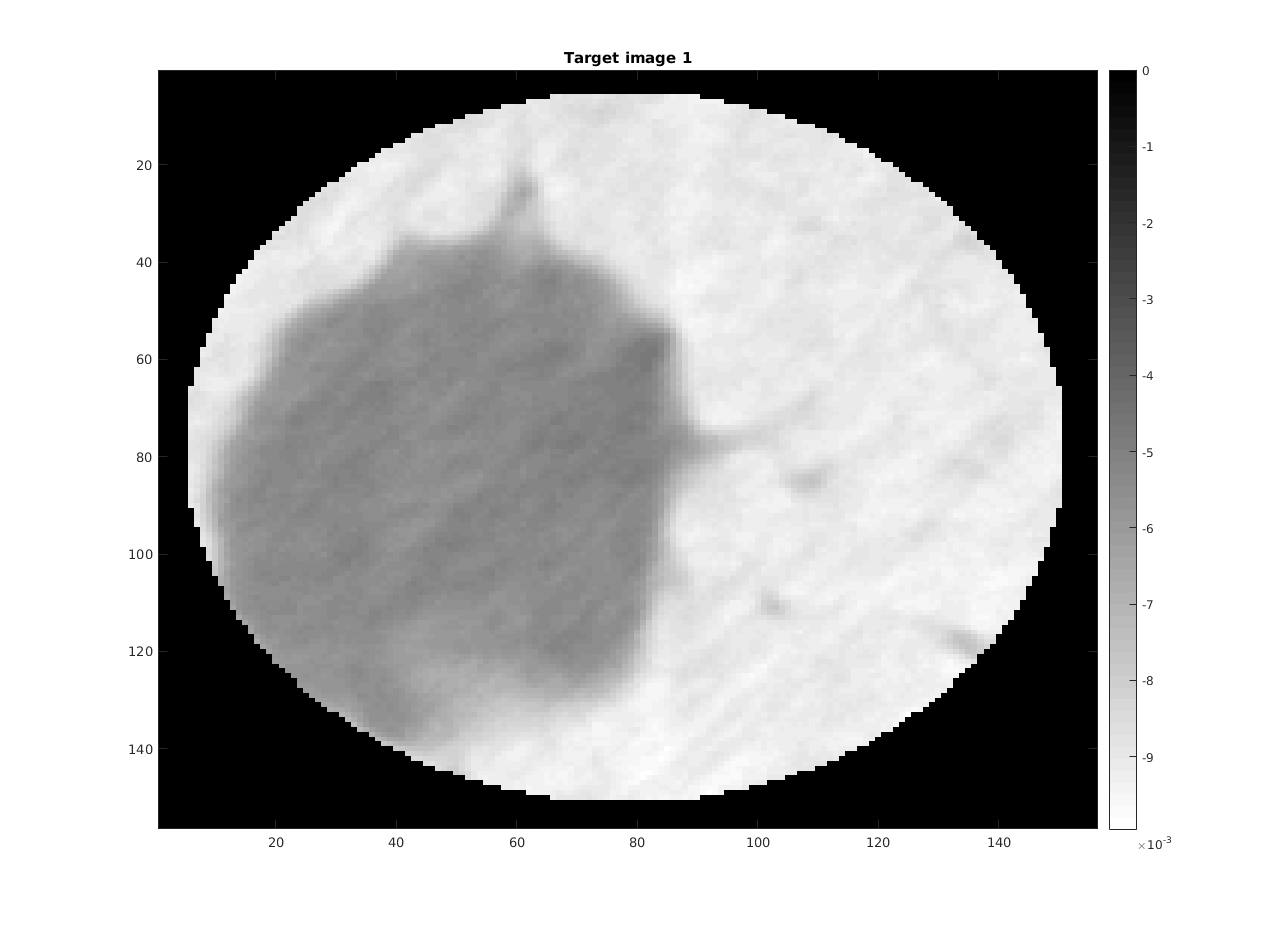
\includegraphics[width=\textwidth]{Sample1/target1.png}
            	\caption{Target image}  
            	%\label{subfig:20it1Fully}
        	\end{subfigure}
        	%\quad
        	\begin{subfigure}[b]{0.32\textwidth}   
        	    \centering 
        	    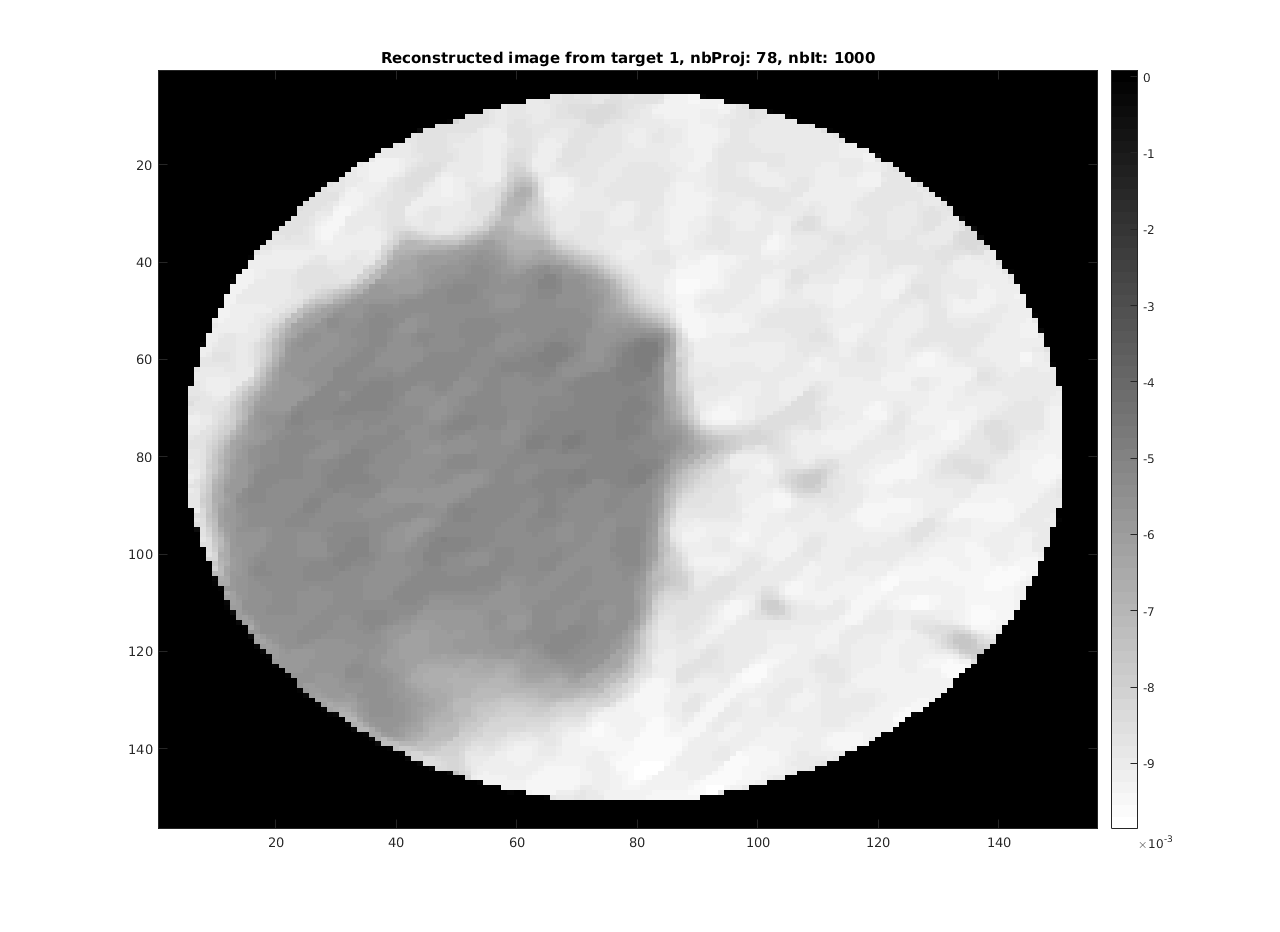
\includegraphics[width=\textwidth]{Sample1/L-D_5000/78_1_2.png}
        	    \caption{78 proj - 50\%}  
        	    \label{subfig:78p1L-D}
       		\end{subfigure}
       		%\hfill
        	\begin{subfigure}[b]{0.32\textwidth}  
            	\centering 
            	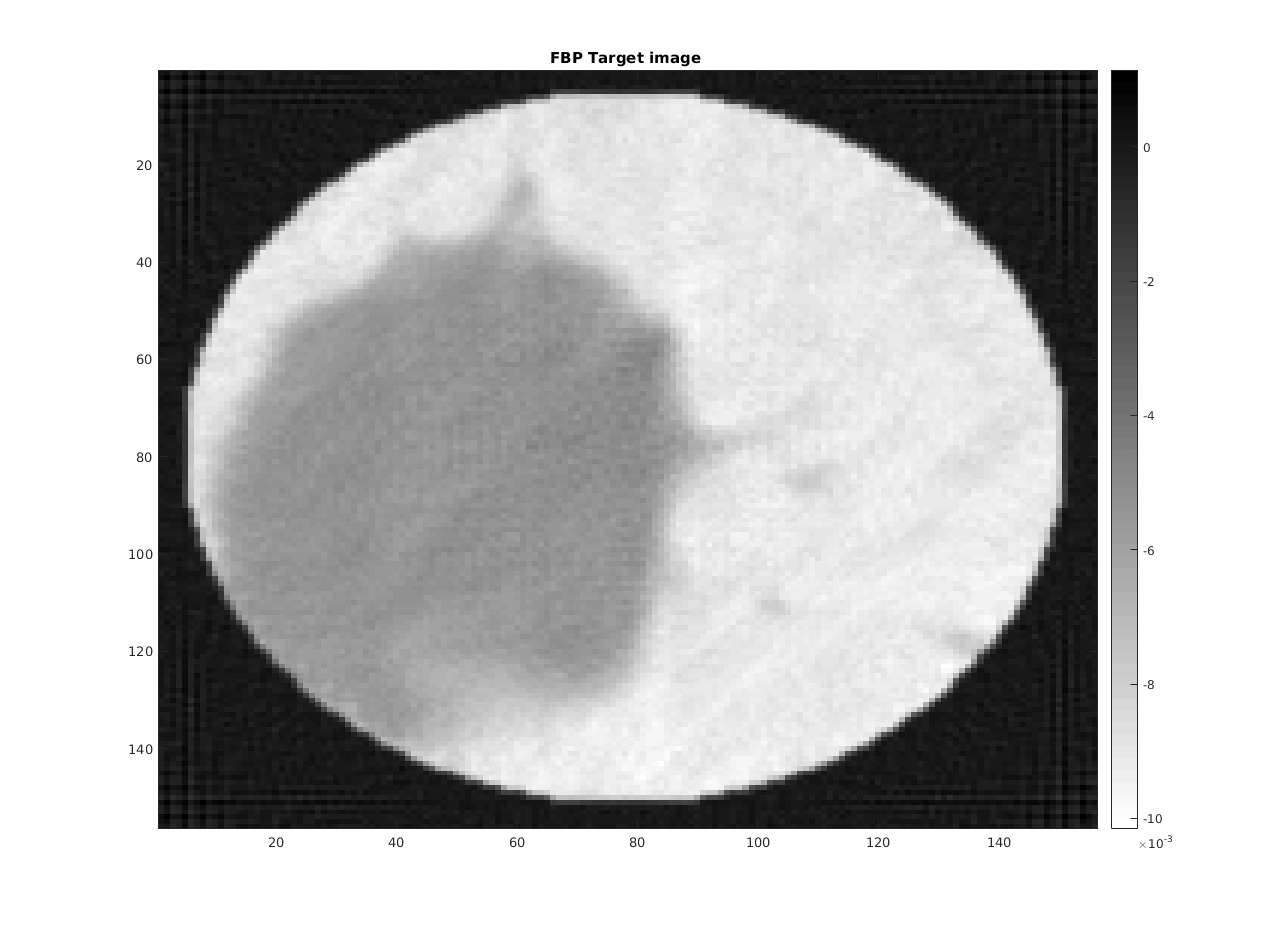
\includegraphics[width=\textwidth]{Sample1/L-D_5000/FBP78.png}
            	\caption{FBP}    
            	\label{subfig:FBP178p}
        	\end{subfigure}
        	\vskip\baselineskip
        	
        	
        	\begin{subfigure}[b]{0.32\textwidth}   
        	    \centering 
            	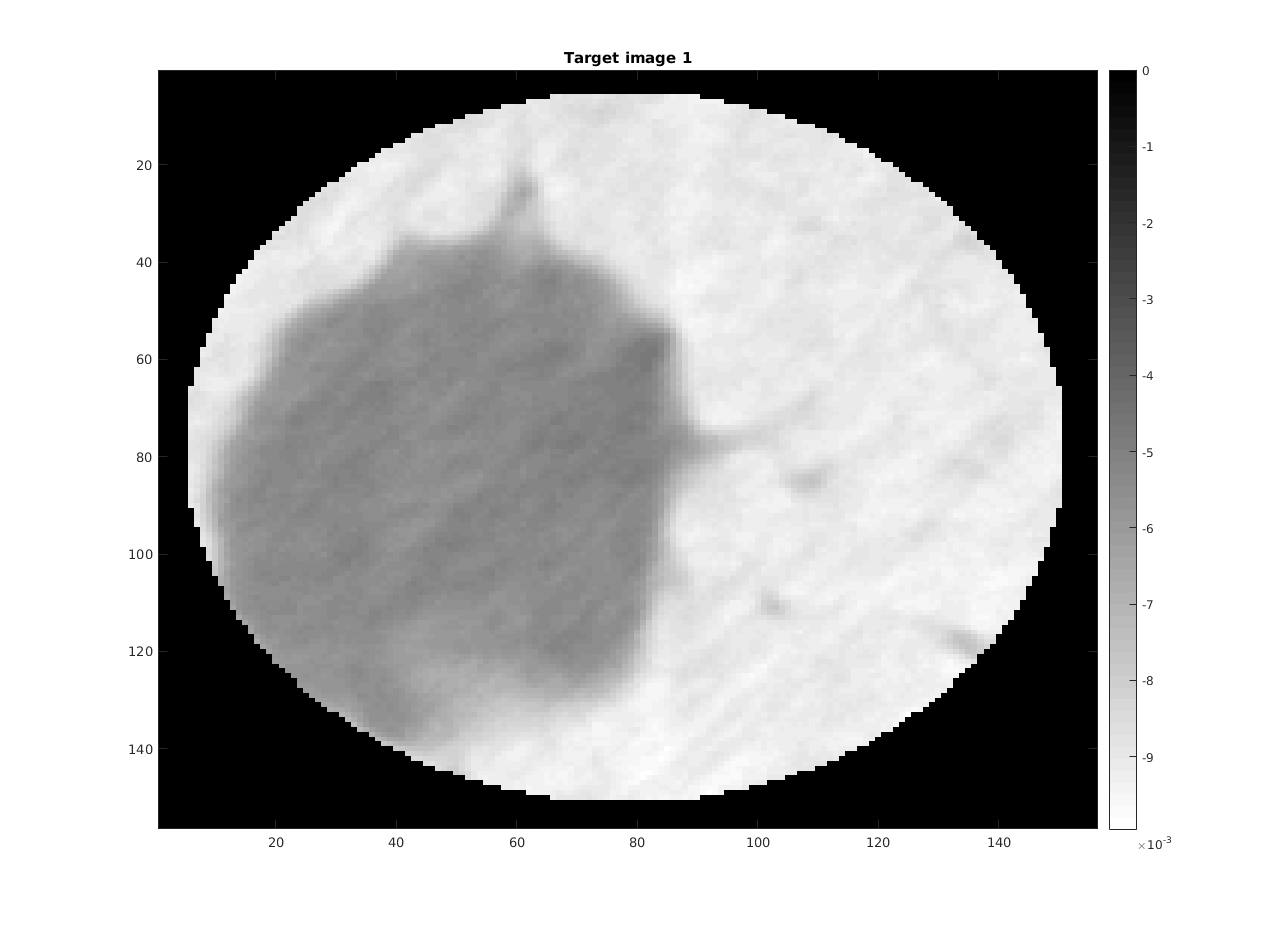
\includegraphics[width=\textwidth]{Sample1/target1.png}
            	\caption{Target image}
            	%\label{subfig:1000it1Fully}
        	\end{subfigure}
        	%\quad
        	\begin{subfigure}[b]{0.32\textwidth}   
        	    \centering 
        	    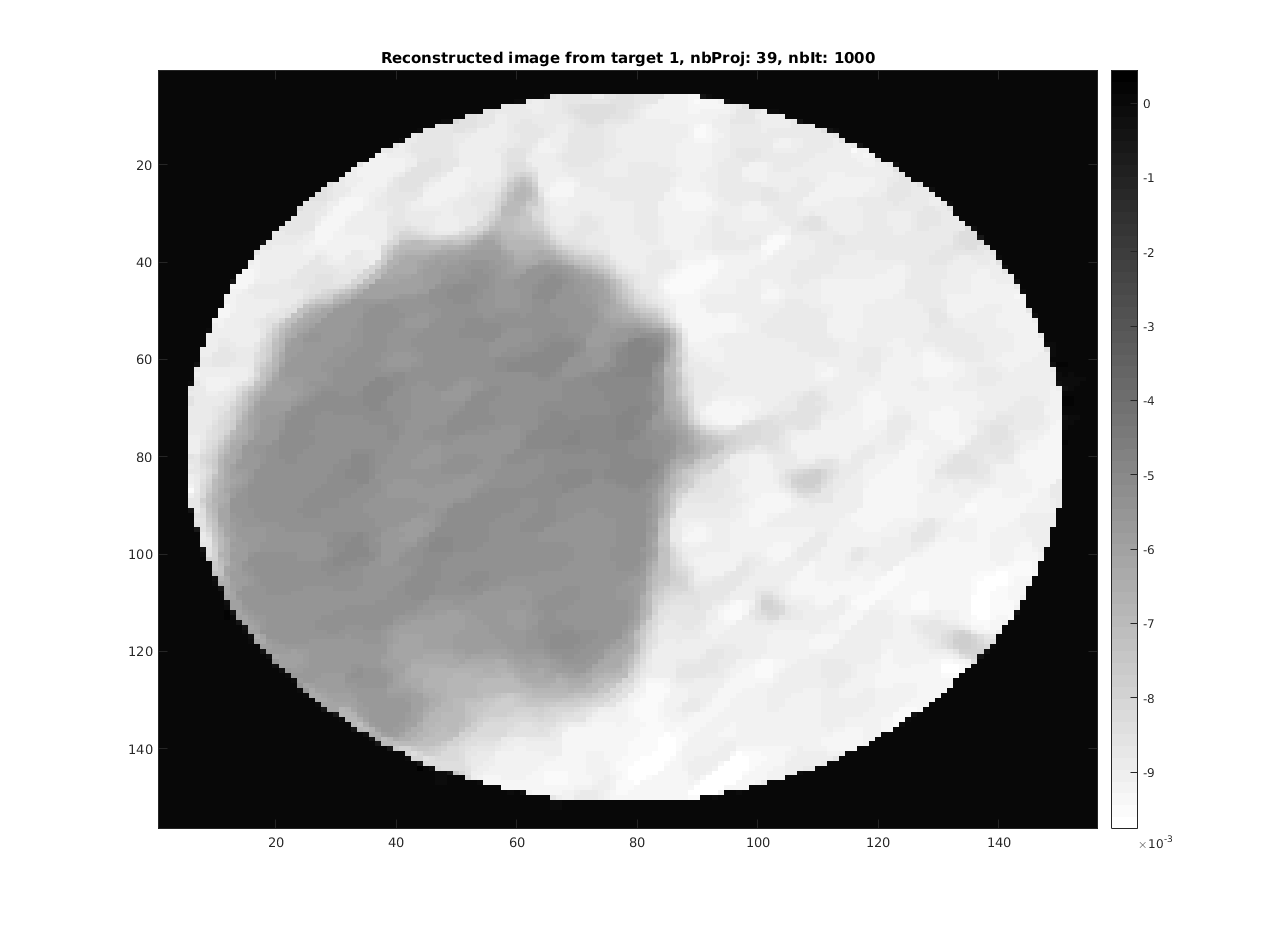
\includegraphics[width=\textwidth]{Sample1/L-D_5000/39_1_4.png}
        	    \caption{39 proj - 25\%}    
        	    \label{subfig:39p1L-D}
       		\end{subfigure}
       		%\hfill
        	\begin{subfigure}[b]{0.32\textwidth}  
            	\centering 
            	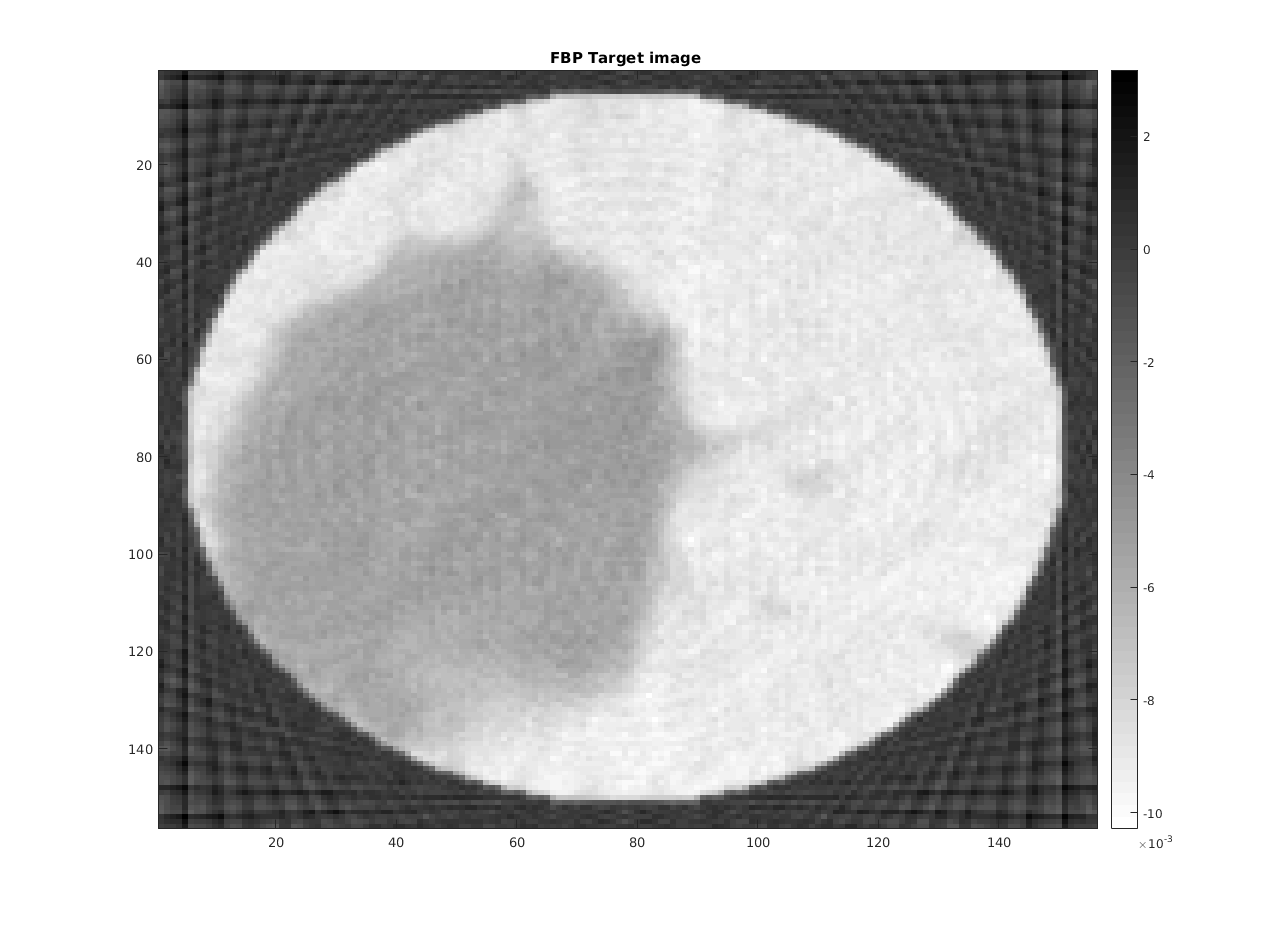
\includegraphics[width=\textwidth]{Sample1/L-D_5000/FBP39.png}
            	\caption{FBP}    
            	\label{subfig:FBP139p}
        	\end{subfigure}
        	\vskip\baselineskip
        	
        	
        	\begin{subfigure}[b]{0.32\textwidth}   
        	    \centering 
            	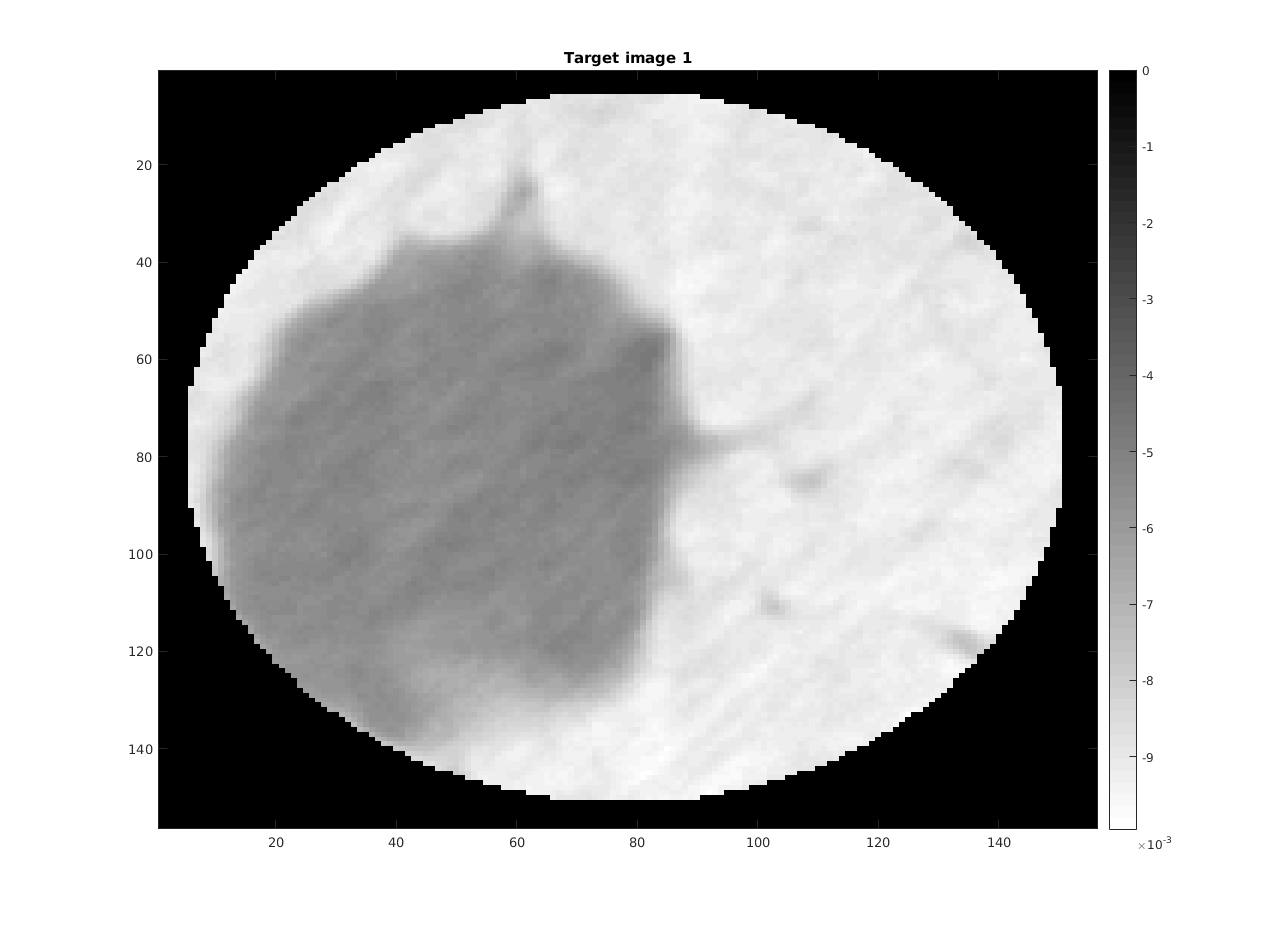
\includegraphics[width=\textwidth]{Sample1/target1.png}
            	\caption{Target image}
            	%\label{subfig:1000it1Fully}
        	\end{subfigure}
        	%\quad
        	\begin{subfigure}[b]{0.32\textwidth}   
        	    \centering 
        	    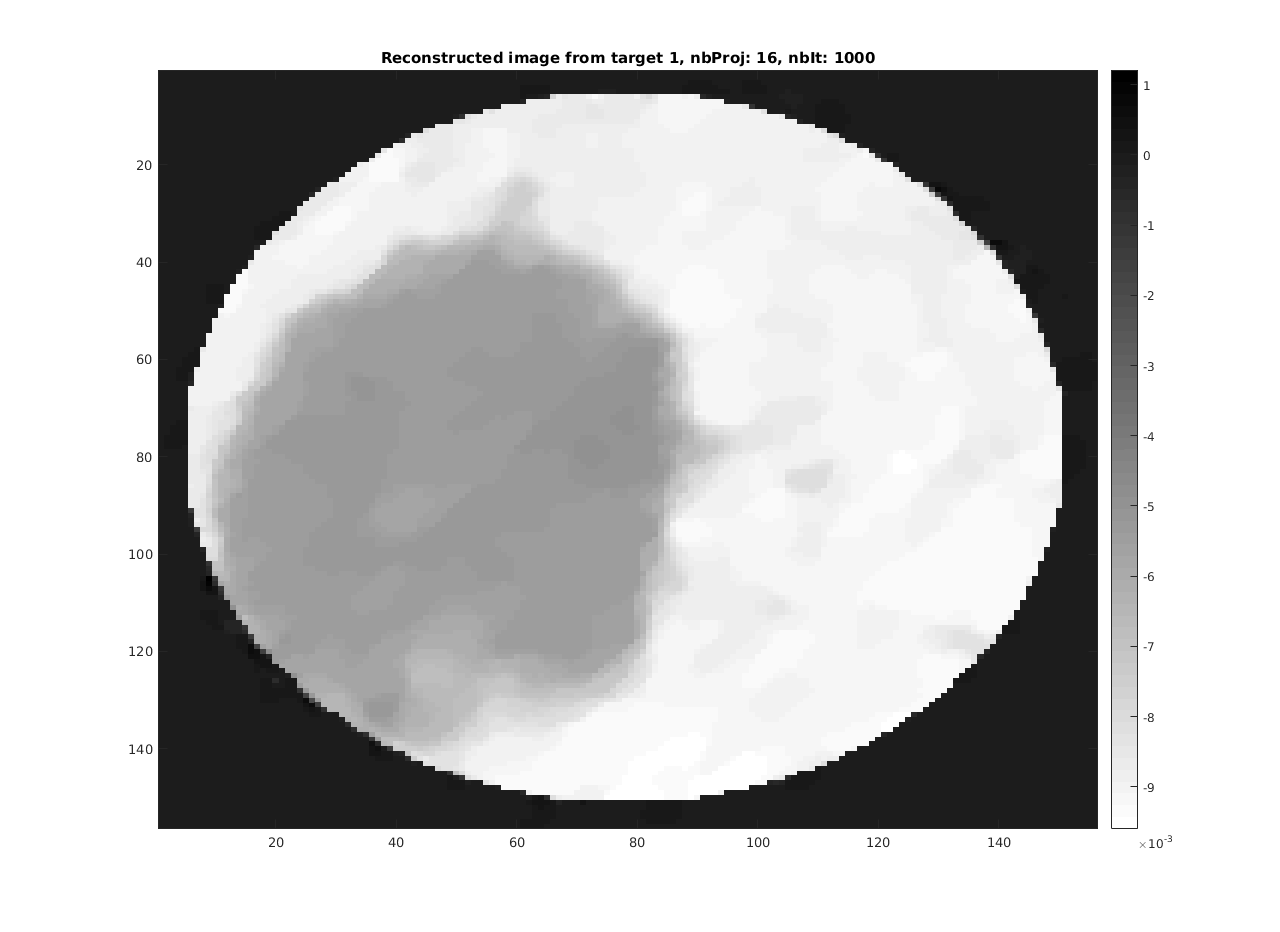
\includegraphics[width=\textwidth]{Sample1/L-D_5000/16_1_10.png}
        	    \caption{16 proj - 10\%}    
        	    \label{subfig:16p1L-D}
       		\end{subfigure}
       		%\hfill
        	\begin{subfigure}[b]{0.32\textwidth}  
            	\centering 
            	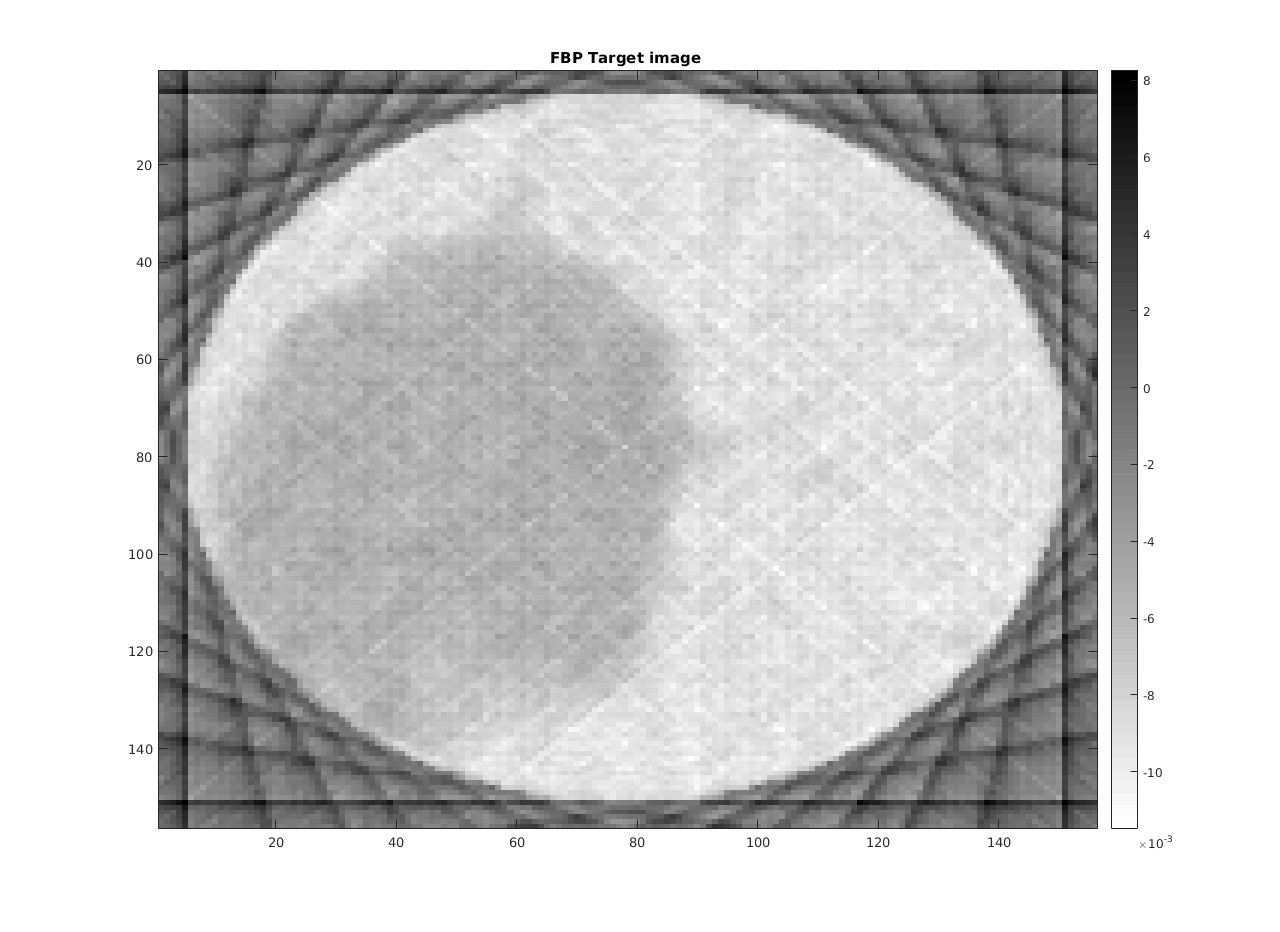
\includegraphics[width=\textwidth]{Sample1/L-D_5000/FBP16.png}
            	\caption{FBP}    
            	\label{subfig:FBP116p}
        	\end{subfigure}
       		
       		
       		
        	\caption{Retro-projections on fully projected object}
        	\label{fig:retFully}
        	
    	\end{figure}
\clearpage

	\subsubsection{Error evaluation}
		in this section we wish to visualize and compare loss of information between Low-Dose SB-TV and FBP as well as define a metric allowing to evaluate the amount of information preserved.\\
		Multiple approaches are proposed.\\	
			
		Table \ref{tab:Error2000Sample1} regroup error evaluations such as normalized variation between reconstructed image and target image. In both of these metrics SB-TV get better results. Although, these methods of error evaluation are less sensitive to noise induced by TV minimization and hence might not be ideal.\\
		
		Peak signal to noise ratio was also evaluated in Table \ref{tab:Error2000Sample1}. This metric is usually  used to measure the compression level of an image compared to a target. Using this method, SB-TV appear to be of a worst quality than FBP. formula: $$ PSNR = 10 \times log_10\left(\frac{MAX_I^2}{MSE}\right)$$\\
		
		Loss of contrast is displayed in Figure \ref{fig:contrastsF1}. This Figure \ref{subfig:ContrastFBP} represents the middle line of FBP reconstruction with different doses when Figure \ref{subfig:ContrastSB} represent SB-TV mid lines. We can notice that FBP preserves the contrast while reducing the number of projections, but results in a noisier signal as the number of projection decrees. SB-TV induces loss of contrast but results in a less noisy signal.\\
		
		We also estimated that one way of evaluating the loss of information would be to work on image edges. To do so we compared canny edge detection on every projections (Figure \ref{fig:Canny}). By applying a threshold of 10\% on the edge detection we were able to isolate the relevant details (Figure \ref{fig:CannyT}). TV of edges detection between target image and reconstructed image is displayed in Table \ref{tab:Error2000Sample1}. \\
		The TV of edges is higher that the TV of images by a factor of $10^3$. Although SB-TV has better results. This gap between image and edges variation come from the fact that edges are shifted between doses even though the information is still there. On idea was then to evaluated the similarities between the images and egdes usinf SIFT descriptor. \\
		SIFT descriptor is scale, rotation and shift invariant. Hence even shifted information will be retrieved and matched to the target image. Figure \ref{fig:SIFTimg} represent SIFT recognition on the images and Figure \ref{fig:SIFTedges} represent SIFT on edges.\\
		Table \ref{tab:SIFT1img} and \ref{tab:SIFT1edges} show that SB-TV preserves more features than FBP which has more confused feature matching.

\clearpage
		\textbf{Canny edges detection}\\
		
		
		\begin{figure}[H]
		
       		\centering
      		\begin{subfigure}[b]{0.32\textwidth}
            	\centering
            	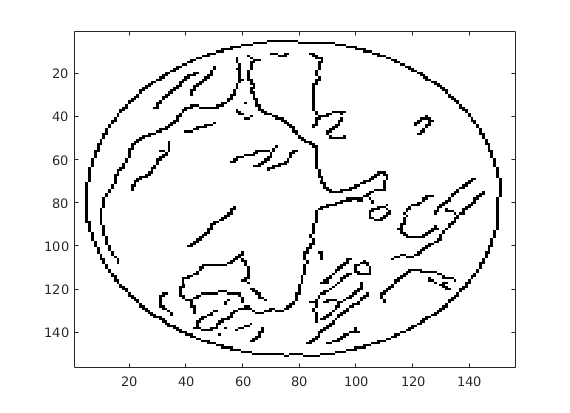
\includegraphics[width=\textwidth]{Sample1/Edges/target_auto.png}
            	\caption{Target image}    
            	%\label{subfig:Target1L-D}
        	\end{subfigure}
        	%\hfill
        	\begin{subfigure}[b]{0.32\textwidth}  
            	\centering 
            	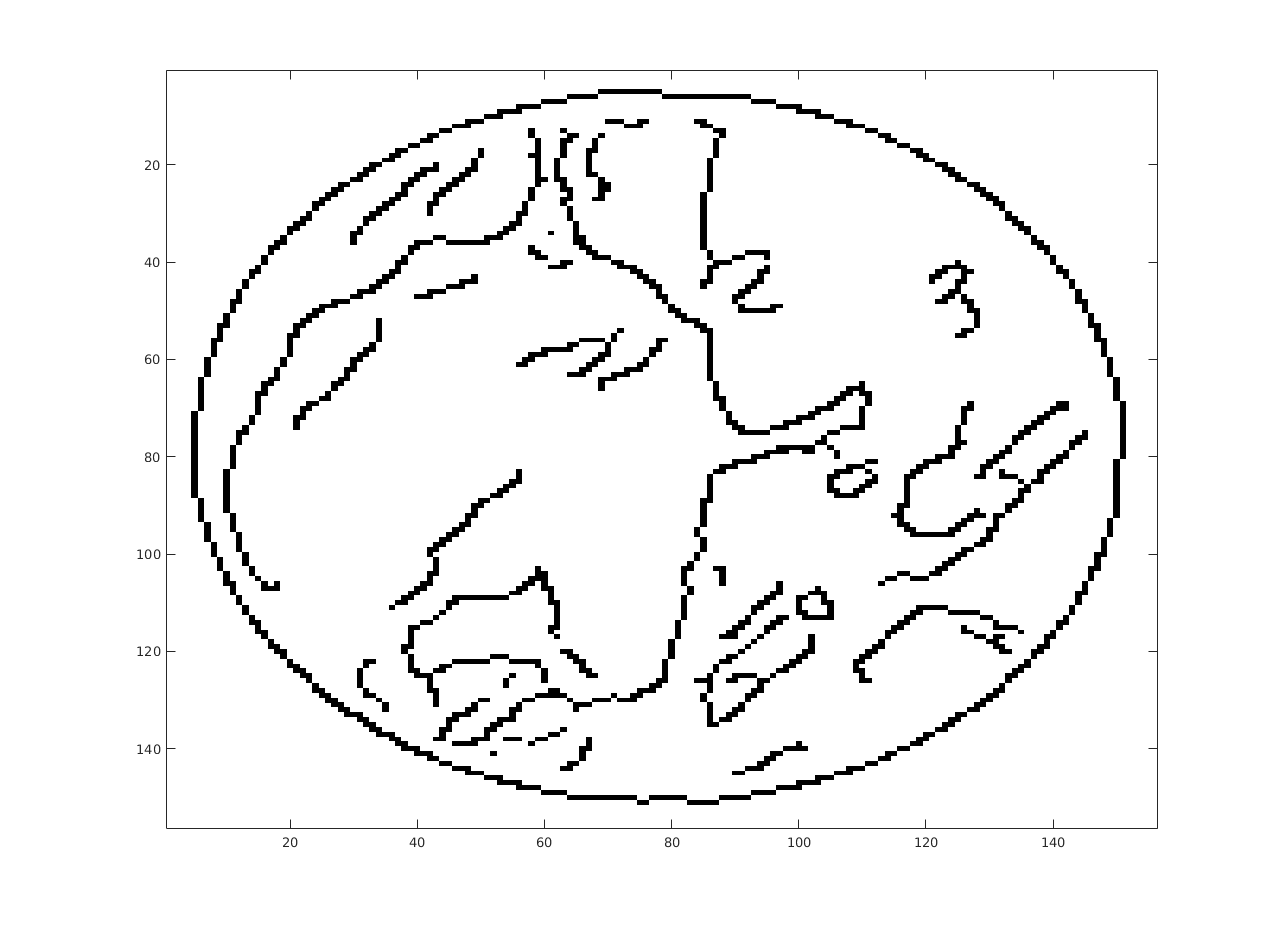
\includegraphics[width=\textwidth]{Sample1/Edges/SB/fully_auto.png}
            	\caption{156 proj - 100\%}    
            	\label{subfig:156p1L-D}
        	\end{subfigure}
        	%\hfill
        	\begin{subfigure}[b]{0.32\textwidth}  
            	\centering 
            	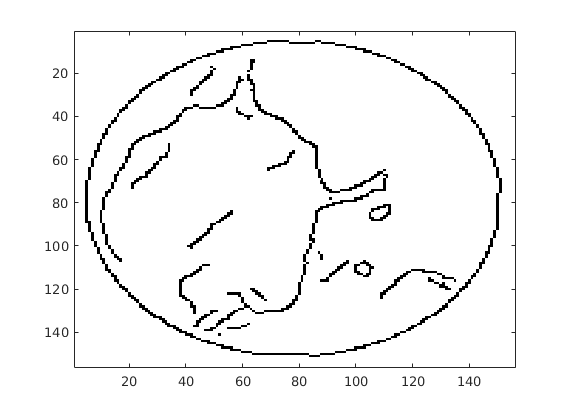
\includegraphics[width=\textwidth]{Sample1/Edges/FBP/fully_auto.png}
            	\caption{FBP}    
            	\label{subfig:FBP1156p}
        	\end{subfigure}
        	\vskip\baselineskip
        	
        	
        	\begin{subfigure}[b]{0.32\textwidth}   
        	    \centering 
            	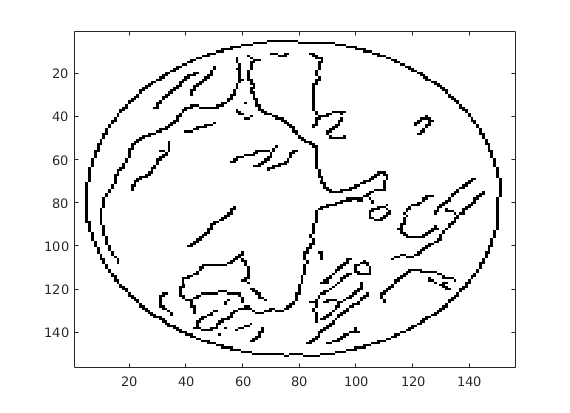
\includegraphics[width=\textwidth]{Sample1/Edges/target_auto.png}
            	\caption{Target image}  
            	%\label{subfig:20it1Fully}
        	\end{subfigure}
        	%\quad
        	\begin{subfigure}[b]{0.32\textwidth}   
        	    \centering 
        	    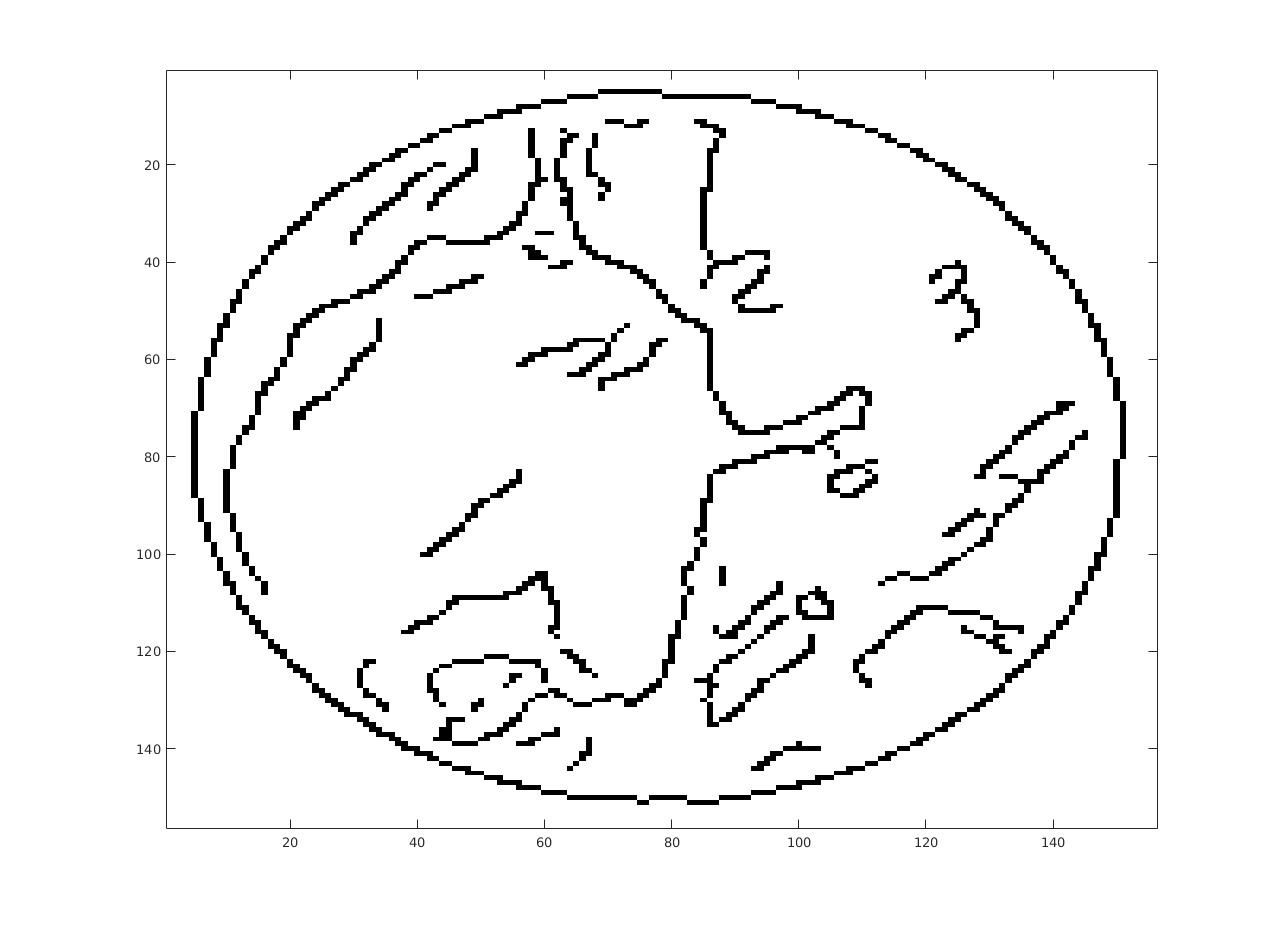
\includegraphics[width=\textwidth]{Sample1/Edges/SB/p2_auto.png}
        	    \caption{78 proj - 50\%}  
        	    \label{subfig:78p1L-D}
       		\end{subfigure}
       		%\hfill
        	\begin{subfigure}[b]{0.32\textwidth}  
            	\centering 
            	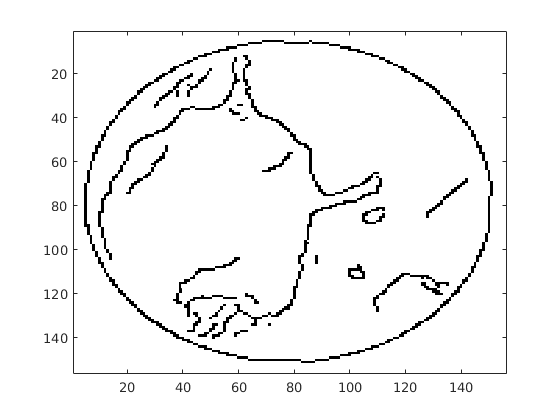
\includegraphics[width=\textwidth]{Sample1/Edges/FBP/p2_auto.png}
            	\caption{FBP}    
            	\label{subfig:FBP178p}
        	\end{subfigure}
        	\vskip\baselineskip
        	
        	
        	\begin{subfigure}[b]{0.32\textwidth}   
        	    \centering 
            	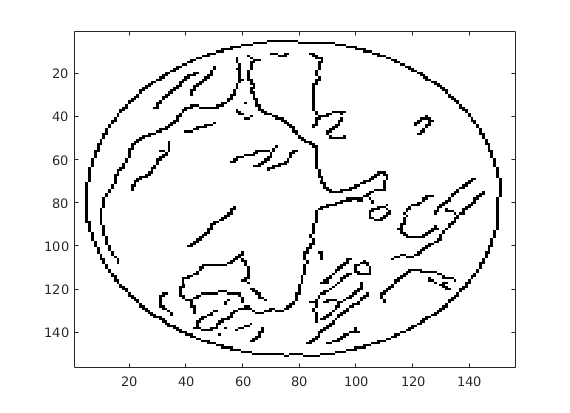
\includegraphics[width=\textwidth]{Sample1/Edges/target_auto.png}
            	\caption{Target image}
            	%\label{subfig:1000it1Fully}
        	\end{subfigure}
        	%\quad
        	\begin{subfigure}[b]{0.32\textwidth}   
        	    \centering 
        	    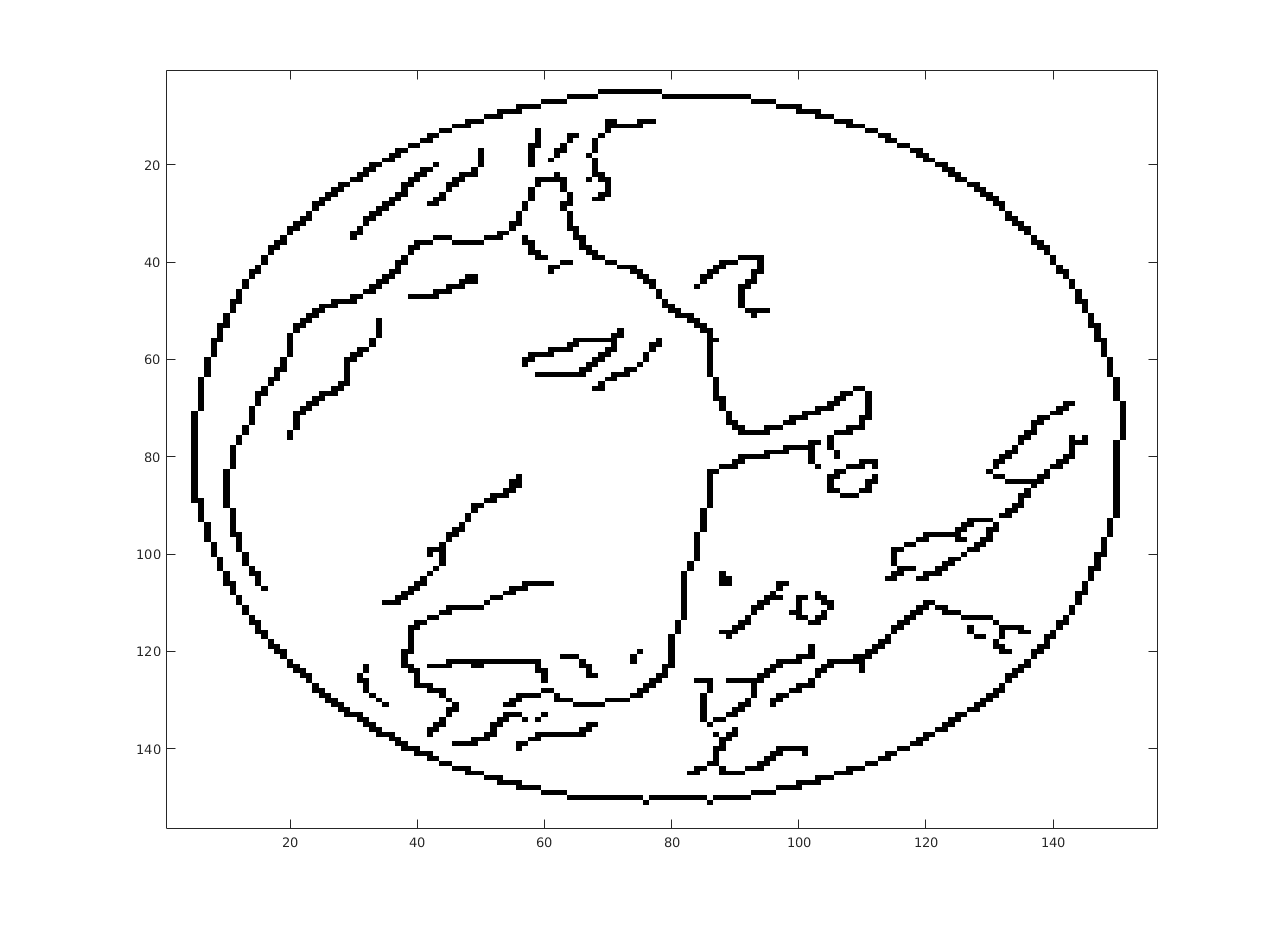
\includegraphics[width=\textwidth]{Sample1/Edges/SB/p3_auto.png}
        	    \caption{39 proj - 25\%}    
        	    \label{subfig:39p1L-D}
       		\end{subfigure}
       		%\hfill
        	\begin{subfigure}[b]{0.32\textwidth}  
            	\centering 
            	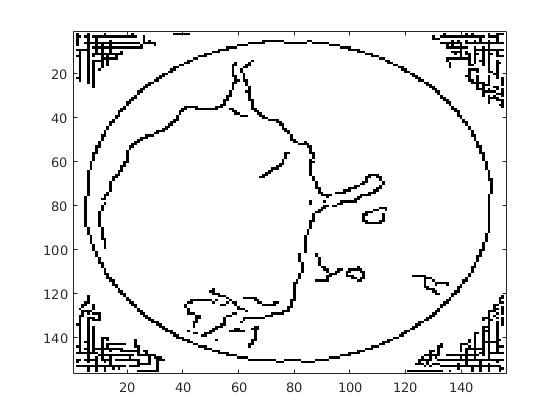
\includegraphics[width=\textwidth]{Sample1/Edges/FBP/p3_auto.png}
            	\caption{FBP}    
            	\label{subfig:FBP139p}
        	\end{subfigure}
        	\vskip\baselineskip
        	
        	
        	\begin{subfigure}[b]{0.32\textwidth}   
        	    \centering 
            	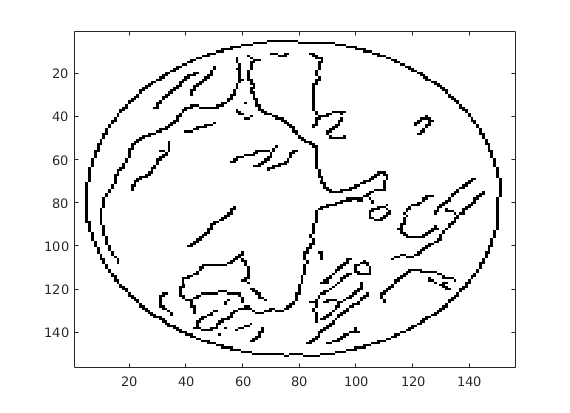
\includegraphics[width=\textwidth]{Sample1/Edges/target_auto.png}
            	\caption{Target image}
            	%\label{subfig:1000it1Fully}
        	\end{subfigure}
        	%\quad
        	\begin{subfigure}[b]{0.32\textwidth}   
        	    \centering 
        	    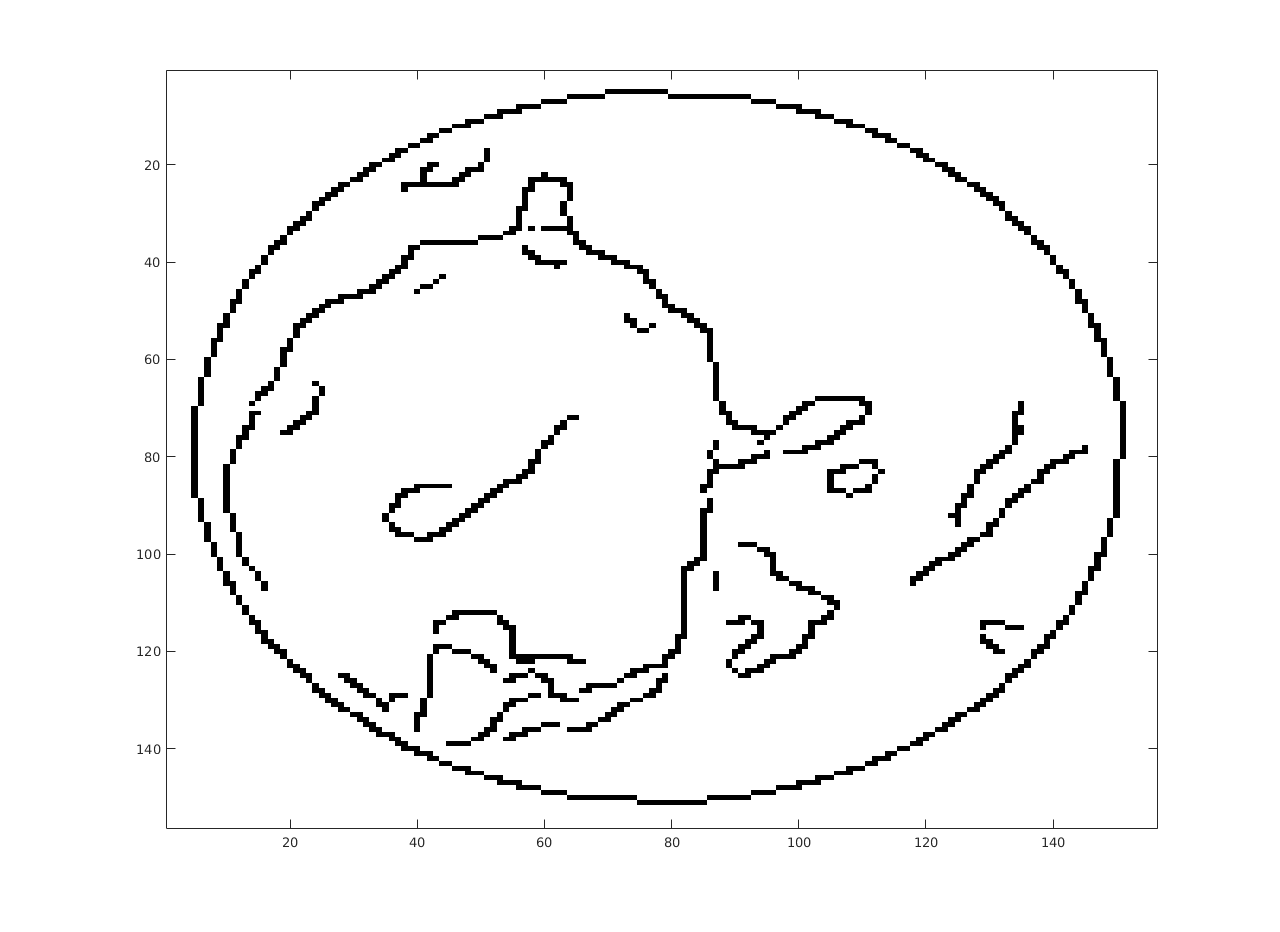
\includegraphics[width=\textwidth]{Sample1/Edges/SB/p4_auto.png}
        	    \caption{16 proj - 10\%}    
        	    \label{subfig:16p1L-D}
       		\end{subfigure}
       		%\hfill
        	\begin{subfigure}[b]{0.32\textwidth}  
            	\centering 
            	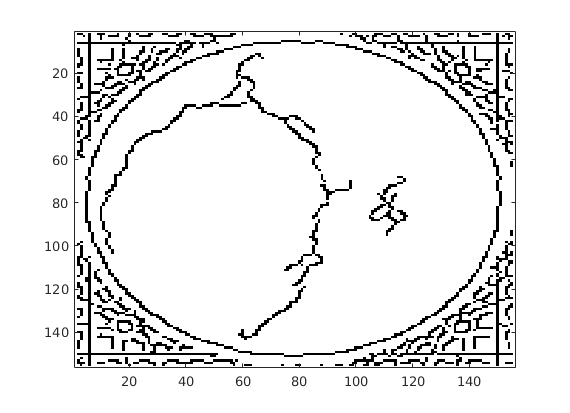
\includegraphics[width=\textwidth]{Sample1/Edges/FBP/p4_auto.png}
            	\caption{FBP}    
            	\label{subfig:FBP116p}
        	\end{subfigure}
       		
       		
       		
        	\caption{Canny edge detection}
        	\label{fig:Canny}
        	
    	\end{figure}

\clearpage
		\textbf{Thresolded Canny edges detection}\\
		The aim to simulate a segmentation. The threshold used is 10\%.
		
		\begin{figure}[H]
		
       		\centering
      		\begin{subfigure}[b]{0.32\textwidth}
            	\centering
            	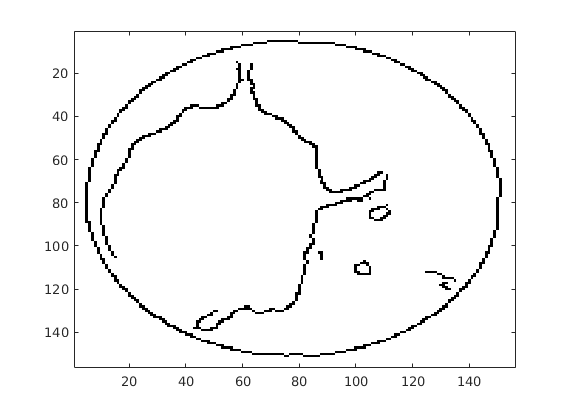
\includegraphics[width=\textwidth]{Sample1/Edges/target_0_10.png}
            	\caption{Target image}    
            	%\label{subfig:Target1L-D}
        	\end{subfigure}
        	%\hfill
        	\begin{subfigure}[b]{0.32\textwidth}  
            	\centering 
            	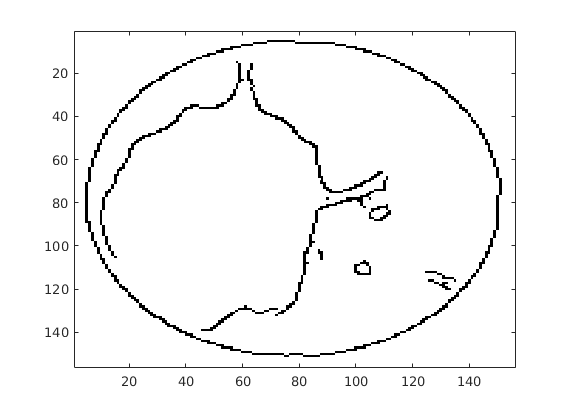
\includegraphics[width=\textwidth]{Sample1/Edges/SB/fully_0_10.png}
            	\caption{156 proj - 100\%}    
            	\label{subfig:156p1L-D}
        	\end{subfigure}
        	%\hfill
        	\begin{subfigure}[b]{0.32\textwidth}  
            	\centering 
            	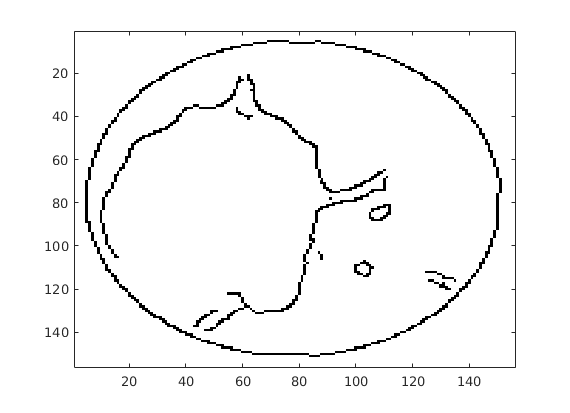
\includegraphics[width=\textwidth]{Sample1/Edges/FBP/fully_0_10.png}
            	\caption{FBP}    
            	\label{subfig:FBP1156p}
        	\end{subfigure}
        	\vskip\baselineskip
        	
        	
        	\begin{subfigure}[b]{0.32\textwidth}   
        	    \centering 
            	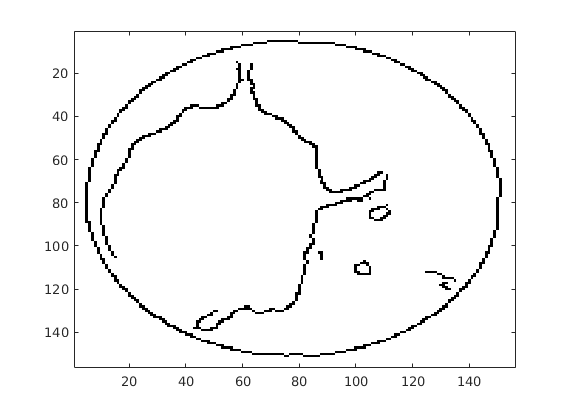
\includegraphics[width=\textwidth]{Sample1/Edges/target_0_10.png}
            	\caption{Target image}  
            	%\label{subfig:20it1Fully}
        	\end{subfigure}
        	%\quad
        	\begin{subfigure}[b]{0.32\textwidth}   
        	    \centering 
        	    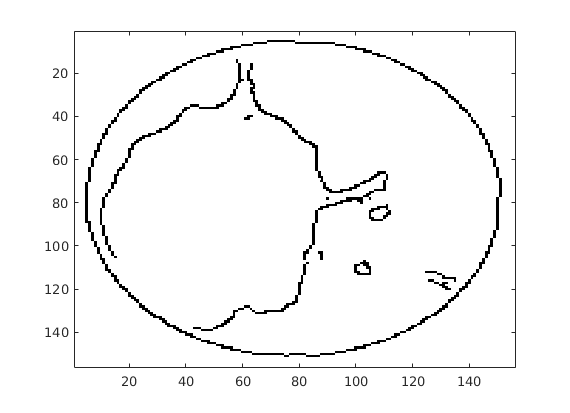
\includegraphics[width=\textwidth]{Sample1/Edges/SB/p2_0_10.png}
        	    \caption{78 proj - 50\%}  
        	    \label{subfig:78p1L-D}
       		\end{subfigure}
       		%\hfill
        	\begin{subfigure}[b]{0.32\textwidth}  
            	\centering 
            	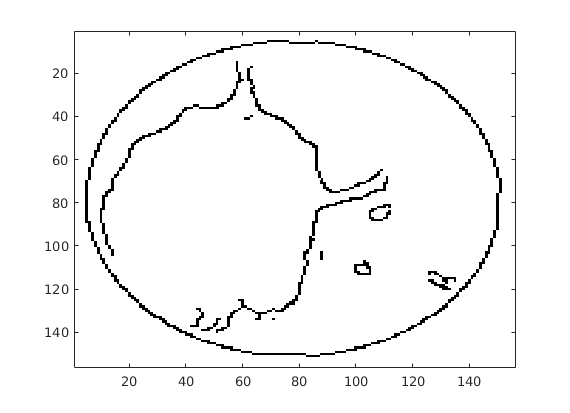
\includegraphics[width=\textwidth]{Sample1/Edges/FBP/p2_0_10.png}
            	\caption{FBP}    
            	\label{subfig:FBP178p}
        	\end{subfigure}
        	\vskip\baselineskip
        	
        	
        	\begin{subfigure}[b]{0.32\textwidth}   
        	    \centering 
            	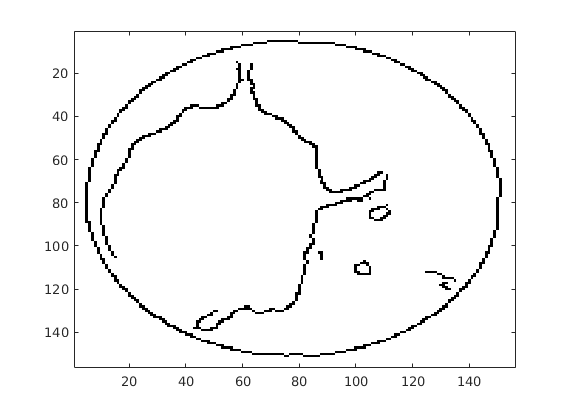
\includegraphics[width=\textwidth]{Sample1/Edges/target_0_10.png}
            	\caption{Target image}
            	%\label{subfig:1000it1Fully}
        	\end{subfigure}
        	%\quad
        	\begin{subfigure}[b]{0.32\textwidth}   
        	    \centering 
        	    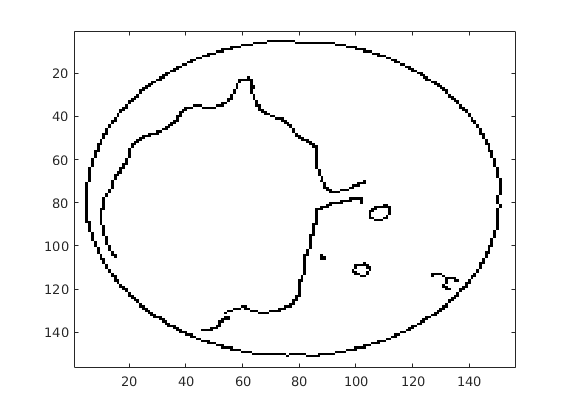
\includegraphics[width=\textwidth]{Sample1/Edges/SB/p3_0_10.png}
        	    \caption{39 proj - 25\%}    
        	    \label{subfig:39p1L-D}
       		\end{subfigure}
       		%\hfill
        	\begin{subfigure}[b]{0.32\textwidth}  
            	\centering 
            	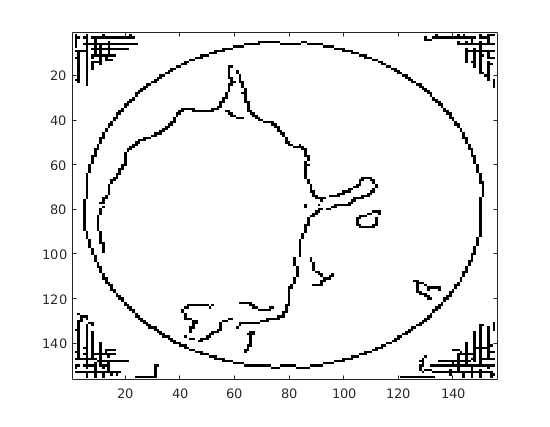
\includegraphics[width=\textwidth]{Sample1/Edges/FBP/p3_0_10.png}
            	\caption{FBP}    
            	\label{subfig:FBP139p}
        	\end{subfigure}
        	\vskip\baselineskip
        	
        	
        	\begin{subfigure}[b]{0.32\textwidth}   
        	    \centering 
            	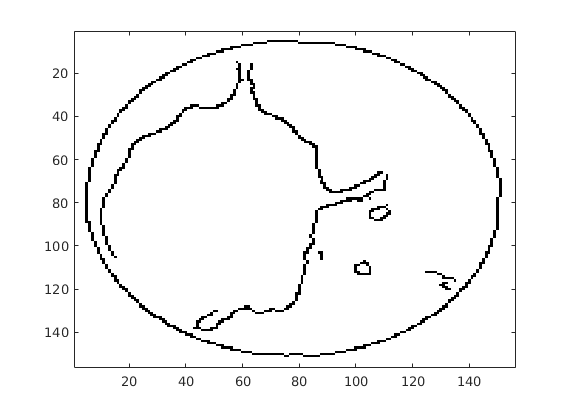
\includegraphics[width=\textwidth]{Sample1/Edges/target_0_10.png}
            	\caption{Target image}
            	%\label{subfig:1000it1Fully}
        	\end{subfigure}
        	%\quad
        	\begin{subfigure}[b]{0.32\textwidth}   
        	    \centering 
        	    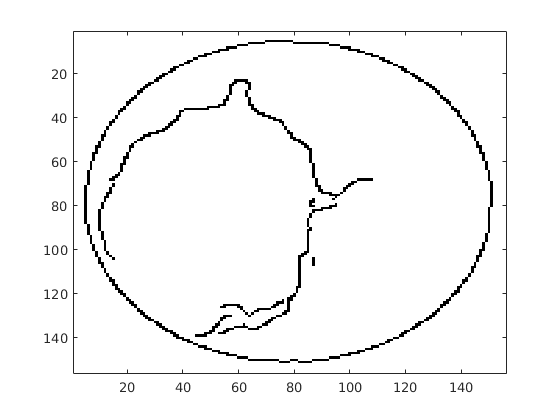
\includegraphics[width=\textwidth]{Sample1/Edges/SB/p4_0_10.png}
        	    \caption{16 proj - 10\%}    
        	    \label{subfig:16p1L-D}
       		\end{subfigure}
       		%\hfill
        	\begin{subfigure}[b]{0.32\textwidth}  
            	\centering 
            	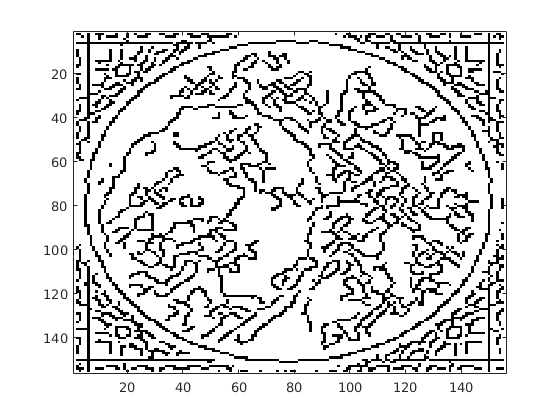
\includegraphics[width=\textwidth]{Sample1/Edges/FBP/p4_0_10.png}
            	\caption{FBP}    
            	\label{subfig:FBP116p}
        	\end{subfigure}
       		
       		
       		
        	\caption{Canny edge detection with threshold of 10\%}
        	\label{fig:CannyT}
        	
    	\end{figure}
    	
\clearpage
		\textbf{Errors table}



		\begin{table}[H]
			\begin{tabular}{ | l || c | c | c | r | }
 				\hline			
   				reconstruction	& 156 Proj (100\%)	& 78 Proj (50\%)	& 39 Proj (25\%)	& 16 Proj (10\%)  \\
   				\hline
  				FBP			    &  $6.00_{e^{-2}}$	& $6.40_{e^{-2}}$	& $8.40_{e^{-2}}$	& $1.86_{e^{-2}}$\\
 				\hline  
 				SB 1000			&  $0.81_{e^{-2}}$  & $0.87_{e^{-2}}$ 	& $1.24_{e^{-2}}$ 	& $2.36_{e^{-2}}$\\
 				\hline 
 				\hline 
				FBP-PSNR		&  68.00			& 67.45				& 65.16				& 58.27\\
				\hline
				SB-PSNR			&  85.54			& 84.84				& 84.8381			& 76.20\\
				\hline
				\hline 
				FBP-TV			&  5.21				& 6.94				& 11.71				& 28.55\\
				\hline
				SB-TV			&  0.91				& 1.01				& 1.40				& 2.07\\
				\hline
				\hline
				FBP-TV-Edges	& $1.115_{e^{+03}}$	& $1.177_{e^{+03}}$	& $2.506_{e^{+03}}$ & $4.259{e^{+03}}$\\
				\hline
				SB-TV-Edges		& $0.378_{e^{+03}}$	& $0.529_{e^{+03}}$	& $1.316_{e^{+03}}$ & $1.969{e^{+03}}$\\
				\hline
								
 				
 			\end{tabular}
 			\caption{Reconstruction error rate from target image}
 			\label{tab:Error2000Sample1}
		\end{table}
		
		\textbf{Contrast loss evaluation}\\
		
		Looking at Figure \ref{fig:contrastsF1} we see that Low-Dose FBP preserves the contrast but adds noise. When Low-Dose SBTV reconstruction is less noisy but loses contrast.
		
		\begin{figure}[H]
			\begin{subfigure}[b]{0.49\textwidth}
				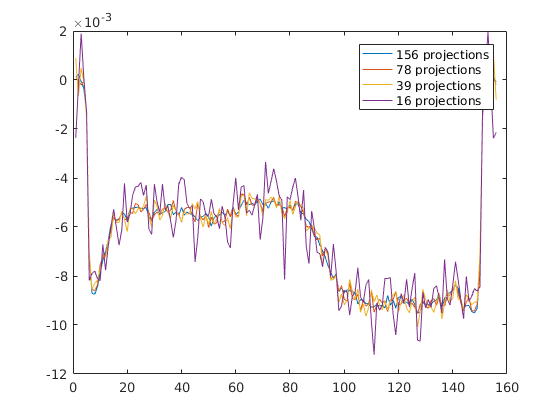
\includegraphics[width=\textwidth]{Sample1/contrastFBP}
				\caption{Contrast of FBP}
				\label{subfig:ContrastFBP}
			\end{subfigure}
			\begin{subfigure}[b]{0.49\textwidth}
				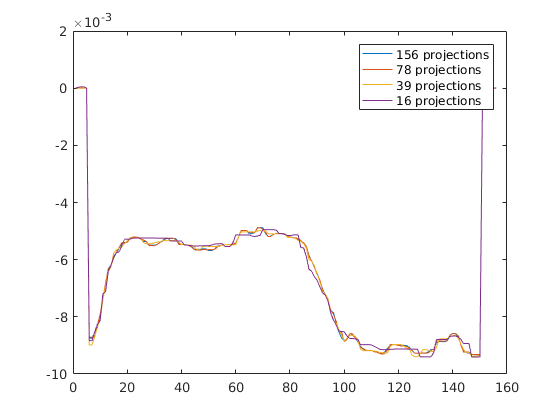
\includegraphics[width=\textwidth]{Sample1/contrastSB}
				\caption{Contrast of SB}
				\label{subfig:ContrastSB}
			\end{subfigure}
			\caption{Contrast of the middle line of sample 1}
			\label{fig:contrastsF1}
		\end{figure}

\clearpage
\textbf{Execution time}\\
				
		\begin{figure}[H]
			\begin{subfigure}[b]{0.49\textwidth}
				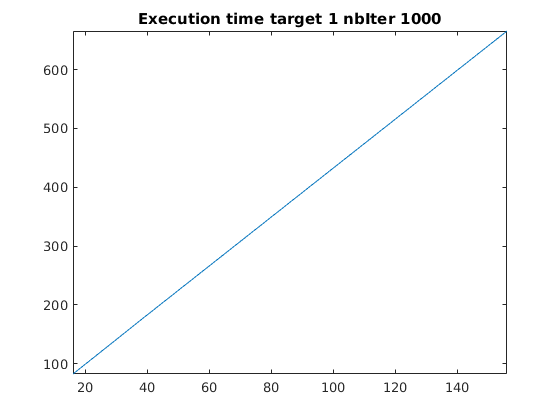
\includegraphics[width=\textwidth]{Sample1/execTimeProj}
				\caption{Execution time: i number of projection, j seconds for 1000 iterations}
				\label{subfig:ContrastFBP}
			\end{subfigure}
			\begin{subfigure}[b]{0.49\textwidth}
				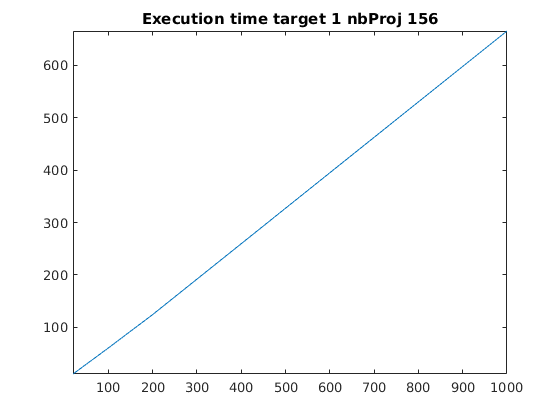
\includegraphics[width=\textwidth]{Sample1/execTimeIt}
				\caption{Execution time: i number of iterations, j seconds for 156 projections (100\%)}
				\label{subfig:ContrastSB}
			\end{subfigure}
			\caption{Execution time of sample 1 156*156 image}
			\label{fig:contrastsF1}
		\end{figure}
		

\begin{figure}
	\begin{figure}[H]
			\begin{subfigure}[b]{0.475\textwidth}
				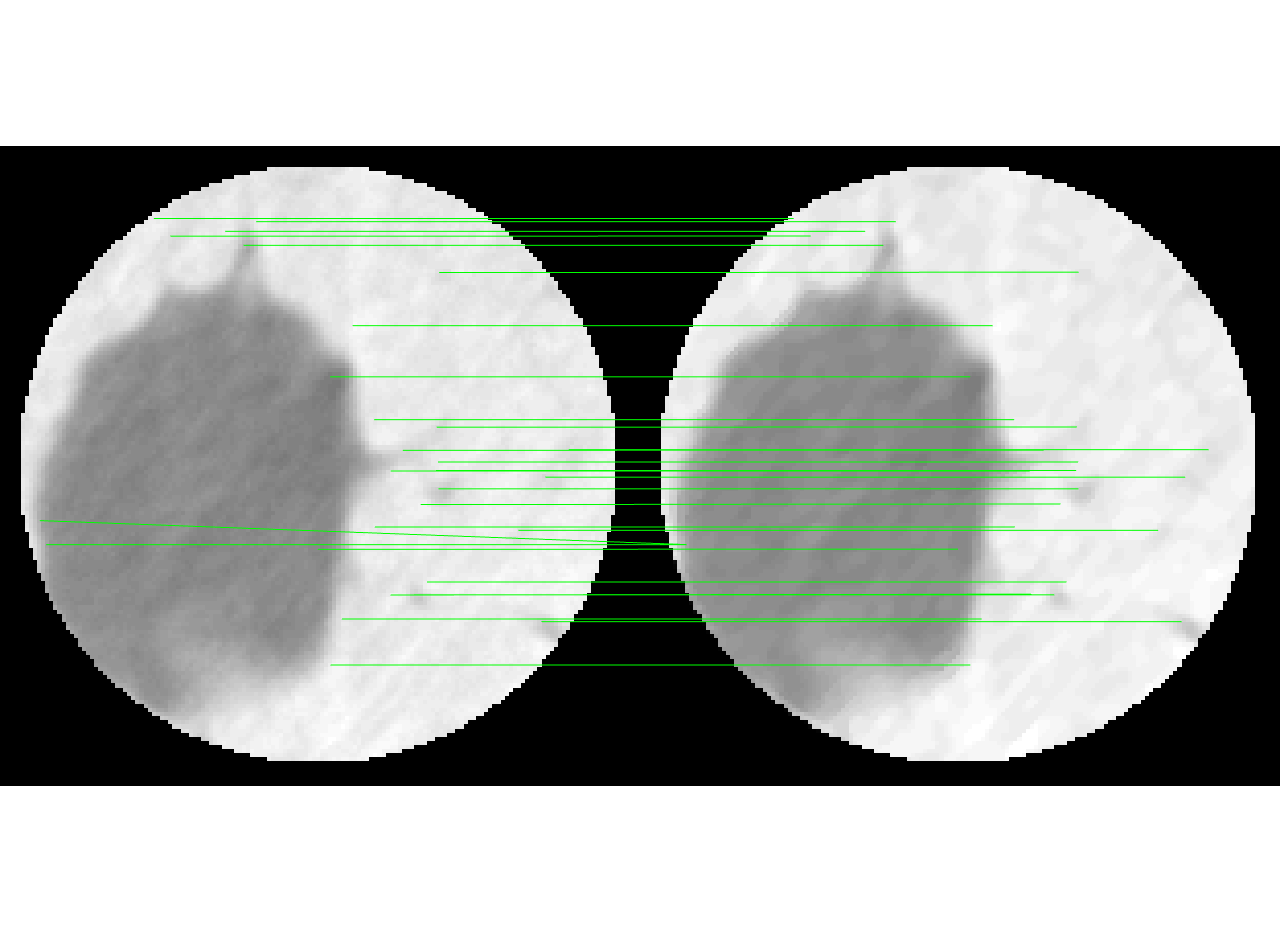
\includegraphics[width=\textwidth]{Sample1/SIFT/SB/100p.png}
				\caption{SIFT SBTV 100\%}
			\end{subfigure}
			\begin{subfigure}[b]{0.475\textwidth}
				\includegraphics[width=\textwidth]{Sample1/SIFT/FBP/100p.png}
				\caption{SIFT FBP 100\%}
			\end{subfigure}
			
			\begin{subfigure}[b]{0.475\textwidth}
				\includegraphics[width=\textwidth]{Sample1/SIFT/SB/50p.png}
				\caption{SIFT SBTV 50\%}
			\end{subfigure}
			\begin{subfigure}[b]{0.475\textwidth}
				\includegraphics[width=\textwidth]{Sample1/SIFT/FBP/50p.png}
				\caption{SIFT FBP 50\%}
			\end{subfigure}
			
			\begin{subfigure}[b]{0.475\textwidth}
				\includegraphics[width=\textwidth]{Sample1/SIFT/SB/25p.png}
				\caption{SIFT SBTV 25\%}
			\end{subfigure}
			\begin{subfigure}[b]{0.475\textwidth}
				\includegraphics[width=\textwidth]{Sample1/SIFT/FBP/25p.png}
				\caption{SIFT FBP 25\%}
			\end{subfigure}
			
			\begin{subfigure}[b]{0.475\textwidth}
				\includegraphics[width=\textwidth]{Sample1/SIFT/SB/10p.png}
				\caption{SIFT SBTV 10\%}
			\end{subfigure}
			\begin{subfigure}[b]{0.475\textwidth}
				\includegraphics[width=\textwidth]{Sample1/SIFT/FBP/10p.png}
				\caption{SIFT FBP 10\%}
			\end{subfigure}
			\caption{SIFT image matching between target and reconstructed images}
			\label{fig:SIFTimg}
		\end{figure}
\end{figure}


\begin{figure}
	\begin{figure}[H]
			\begin{subfigure}[b]{0.475\textwidth}
				\includegraphics[width=\textwidth]{Sample1/SIFT/Edges/SB/100p.png}
				\caption{SIFT SBTV 100\%}
			\end{subfigure}
			\begin{subfigure}[b]{0.475\textwidth}
				\includegraphics[width=\textwidth]{Sample1/SIFT/Edges/FBP/100p.png}
				\caption{SIFT FBP 100\%}
			\end{subfigure}
			
			\begin{subfigure}[b]{0.475\textwidth}
				\includegraphics[width=\textwidth]{Sample1/SIFT/Edges/SB/50p.png}
				\caption{SIFT SBTV 50\%}
			\end{subfigure}
			\begin{subfigure}[b]{0.475\textwidth}
				\includegraphics[width=\textwidth]{Sample1/SIFT/Edges/FBP/50p.png}
				\caption{SIFT FBP 50\%}
			\end{subfigure}
			
			\begin{subfigure}[b]{0.475\textwidth}
				\includegraphics[width=\textwidth]{Sample1/SIFT/Edges/SB/25p.png}
				\caption{SIFT SBTV 25\%}
			\end{subfigure}
			\begin{subfigure}[b]{0.475\textwidth}
				\includegraphics[width=\textwidth]{Sample1/SIFT/Edges/FBP/25p.png}
				\caption{SIFT FBP 25\%}
			\end{subfigure}
			
			\begin{subfigure}[b]{0.475\textwidth}
				\includegraphics[width=\textwidth]{Sample1/SIFT/Edges/SB/10p.png}
				\caption{SIFT SBTV 10\%}
			\end{subfigure}
			\begin{subfigure}[b]{0.475\textwidth}
				\includegraphics[width=\textwidth]{Sample1/SIFT/Edges/FBP/10p.png}
				\caption{SIFT FBP 10\%}
			\end{subfigure}
			\caption{SIFT image matching between target and reconstructed images edges}
			\label{fig:SIFTedges}
		\end{figure}
\end{figure}
\clearpage


		\begin{table}[H]
			\begin{tabular}{ | l | c | c || c | c | r | }
 				\hline			
   				reconstruction	& matches		& FP			& Reconstuction	&  matches 	& FP  \\
   				\hline
  				SB 100\%	    &  37			& 2 (5.41\%)	& FBP 100\%			& 28	& 6 (21.43\%)\\
 				\hline  
 				SB 50\%			&  37			& 1	(2.70\%)	& FBP 50\%			& 32	& 3 (9.38\%)\\
 				\hline 
 				SB 25\%			&  24			& 1	(4.17\%)	& FBP 25\%			& 23	& 4 (17.39\%)\\
				\hline
				SB 10 \%		&  13			& 3	(23.08\%)	& FBP 10\%			& 8		& 3 (37.50\%)\\
				\hline
	 				
 			\end{tabular}
 			\caption{SIFT image matching}
 			\label{tab:SIFT1img}
		\end{table}
		
		\begin{table}[H]
			\begin{tabular}{ | l | c | c || c | c | r | }
 				\hline			
   				reconstruction	& matches		& FP			& Reconstuction	&  matches 	& FP  \\
   				\hline
  				SB 100\%	    &  72			& 4 (5.56\%)	& FBP 100\%		& 16		& 4 (25\%)\\
 				\hline  
 				SB 50\%			&  52			& 6	(11.54\%)	& FBP 50\%		& 13		& 1 (7,69\%)\\
 				\hline 
 				SB 25\%			&  22			& 2	(9.09\%)	& FBP 25\%		& 8			& 3 (37.5\%)\\
				\hline
				SB 10 \%		&  14			& 8	(57,14\%)	& FBP 10\%		& 1			& 1 (100\%)\\
				\hline
	 				
 			\end{tabular}
 			\caption{SIFT Edges matching}
 			\label{tab:SIFT1edges}
		\end{table}


	\subsection{Image sample 2}
		\subsubsection{Fully projected}
			%Use of 156 projections. We are here comparing the number of iterations of Split Bregman algorithm to the target and FBP images (respectively Figure \ref{subfig:Target2Fully} and \ref{subfig:FBP2Fully}. in Figure \ref{fig:retFully} are displayed 20, 200, 1000 and 5000 iterations.\\
			%We can notice that the number of edges recovered increases with the number of iterations.\\
			%In the next sections we will use 5000 iterations since it corresponds to the best image recovery.
			%Some evaluation metrics are displayed in Table \ref{tab:Error2000Sample2}
		\begin{figure}[H]
		
       		\centering
      		\begin{subfigure}[b]{0.475\textwidth}
            	\centering
            	\includegraphics[width=\textwidth]{Sample2/target2.png}
            	\caption{Target image}    
            	\label{subfig:Target2Fully}
        	\end{subfigure}
        	\hfill
        	\begin{subfigure}[b]{0.475\textwidth}  
            	\centering 
            	\includegraphics[width=\textwidth]{Sample2/fully/FBP.png}
            	\caption{FBP}    
            	\label{subfig:FBP2Fully}
        	\end{subfigure}
        	\vskip\baselineskip
        	\begin{subfigure}[b]{0.475\textwidth}   
        	    \centering 
            	\includegraphics[width=\textwidth]{Sample2/fully/20it.png}
            	\caption{SB 20}  
            	\label{subfig:20it1Fully}
        	\end{subfigure}
        	\quad
        	\begin{subfigure}[b]{0.475\textwidth}   
        	    \centering 
        	    \includegraphics[width=\textwidth]{Sample2/fully/200it.png}
        	    \caption{SB 200}  
        	    \label{subfig:200it1Fully}
       		\end{subfigure}
        	\vskip\baselineskip
        	\begin{subfigure}[b]{0.475\textwidth}   
        	    \centering 
            	\includegraphics[width=\textwidth]{Sample2/fully/1000it.png}
            	\caption{SB 1000}
            	\label{subfig:1000it1Fully}
        	\end{subfigure}
        	\quad
        	\begin{subfigure}[b]{0.475\textwidth}   
        	    \centering 
        	    \includegraphics[width=\textwidth]{Sample2/fully/5000it.png}
        	    \caption{SB 5000}    
        	    \label{subfig:5000it1Fully}
       		\end{subfigure}
        	\caption{Retro-projections on fully projected object}
        	\label{fig:retFully}
    	\end{figure}

		\begin{table}[H]
			\begin{tabular}{ | l || c || c | c | c | c | r | }
 				\hline			
   				reconstruction	& FBP 	& SB 5000	& SB 1000	& SB 200	& SB 100	& SB 20 \\
   				\hline
  				Error			& 0.058	& 0.0116	& 0.0124	& 0.0176	& 0.0292	& 0.1059 \\
 				\hline  
 				Time exec		&		& 11.96		& 62.45		& 129.66	& 647.87	& 3314	\\
 				\hline 
 			\end{tabular}
 			\caption{Reconstruction error rate from target image}
 			\label{tab:Error2000Sample2}
		\end{table}
\clearpage		
		\subsubsection{Sample 2 Low-Dose reconstruction}
		\begin{figure}[H]
		
       		\centering
      		\begin{subfigure}[b]{0.32\textwidth}
            	\centering
            	\includegraphics[width=\textwidth]{Sample2/target2.png}
            	\caption{Target image}    
            	%\label{subfig:Target2L-D}
        	\end{subfigure}
        	%\hfill
        	\begin{subfigure}[b]{0.32\textwidth}  
            	\centering 
            	\includegraphics[width=\textwidth]{Sample2/L-D_5000/156p.png}
            	\caption{156 proj - 100\%}    
            	\label{subfig:156p2L-D}
        	\end{subfigure}
        	%\hfill
        	\begin{subfigure}[b]{0.32\textwidth}  
            	\centering 
            	\includegraphics[width=\textwidth]{Sample2/L-D_5000/FBP156.png}
            	\caption{FBP}    
            	\label{subfig:FBP2156p}
        	\end{subfigure}
        	\vskip\baselineskip
        	
        	
        	\begin{subfigure}[b]{0.32\textwidth}   
        	    \centering 
            	\includegraphics[width=\textwidth]{Sample2/target2.png}
            	\caption{Target image}  
            	%\label{subfig:20it1Fully}
        	\end{subfigure}
        	%\quad
        	\begin{subfigure}[b]{0.32\textwidth}   
        	    \centering 
        	    \includegraphics[width=\textwidth]{Sample2/L-D_5000/78_1_2.png}
        	    \caption{78 proj - 50\%}  
        	    \label{subfig:78p2L-D}
       		\end{subfigure}
       		%\hfill
        	\begin{subfigure}[b]{0.32\textwidth}  
            	\centering 
            	\includegraphics[width=\textwidth]{Sample2/L-D_5000/FBP78.png}
            	\caption{FBP}    
            	\label{subfig:FBP278p}
        	\end{subfigure}
        	\vskip\baselineskip
        	
        	
        	\begin{subfigure}[b]{0.32\textwidth}   
        	    \centering 
            	\includegraphics[width=\textwidth]{Sample2/target2.png}
            	\caption{Target image}
            	%\label{subfig:1000it1Fully}
        	\end{subfigure}
        	%\quad
        	\begin{subfigure}[b]{0.32\textwidth}   
        	    \centering 
        	    \includegraphics[width=\textwidth]{Sample2/L-D_5000/39_1_4.png}
        	    \caption{39 proj - 25\%}    
        	    \label{subfig:39p2L-D}
       		\end{subfigure}
       		%\hfill
        	\begin{subfigure}[b]{0.32\textwidth}  
            	\centering 
            	\includegraphics[width=\textwidth]{Sample2/L-D_5000/FBP39.png}
            	\caption{FBP}    
            	\label{subfig:FBP239p}
        	\end{subfigure}
        	\vskip\baselineskip
        	
        	
        	\begin{subfigure}[b]{0.32\textwidth}   
        	    \centering 
            	\includegraphics[width=\textwidth]{Sample2/target2.png}
            	\caption{Target image}
            	%\label{subfig:1000it1Fully}
        	\end{subfigure}
        	%\quad
        	\begin{subfigure}[b]{0.32\textwidth}   
        	    \centering 
        	    \includegraphics[width=\textwidth]{Sample2/L-D_5000/16_1_10.png}
        	    \caption{16 proj - 10\%}    
        	    \label{subfig:16p2L-D}
       		\end{subfigure}
       		%\hfill
        	\begin{subfigure}[b]{0.32\textwidth}  
            	\centering 
            	\includegraphics[width=\textwidth]{Sample2/L-D_5000/FBP16.png}
            	\caption{FBP}    
            	\label{subfig:FBP216p}
        	\end{subfigure}
       		
       		
       		
        	\caption{Retro-projections on fully projected object}
        	\label{fig:retFully}
        	
    	\end{figure}

		\begin{table}[H]
			\begin{tabular}{ | l || c | c | c | r | }
 				\hline			
   				reconstruction	& 156 Proj (100\%)	& 78 Proj (50\%)	& 39 Proj (25\%)	& 16 Proj (10\%)  \\
   				\hline
  				FBP			    &  0.058			& 0.062				& 0.084				& 0.200\\
 				\hline  
 				SB 5000			&  0.012			& 0.013				& 0.019				& 0.049\\
 				\hline 
 			\end{tabular}
 			\caption{Reconstruction error rate from target image}
 			\label{tab:Error2000Sample2}
		\end{table}

\clearpage

	\subsection{Image sample 3}
		\subsubsection{Fully projected (image size \#proj)}
		\begin{figure}[H]
		
       		\centering
      		\begin{subfigure}[b]{0.475\textwidth}
            	\centering
            	\includegraphics[width=\textwidth]{Sample3/target3.png}
            	\caption{Target image}    
            	\label{subfig:Target1Fully}
        	\end{subfigure}
        	\hfill
        	\begin{subfigure}[b]{0.475\textwidth}  
            	\centering 
            	\includegraphics[width=\textwidth]{Sample3/fully/FBP.png}
            	\caption{FBP}    
            	\label{subfig:FBP3Fully}
        	\end{subfigure}
        	\vskip\baselineskip
        	\begin{subfigure}[b]{0.475\textwidth}   
        	    \centering 
            	\includegraphics[width=\textwidth]{Sample3/fully/20it.png}
            	\caption{SB 20}  
            	\label{subfig:20it1Fully}
        	\end{subfigure}
        	\quad
        	\begin{subfigure}[b]{0.475\textwidth}   
        	    \centering 
        	    \includegraphics[width=\textwidth]{Sample3/fully/200it.png}
        	    \caption{SB 200}  
        	    \label{subfig:200it1Fully}
       		\end{subfigure}
        	\vskip\baselineskip
        	\begin{subfigure}[b]{0.475\textwidth}   
        	    \centering 
            	\includegraphics[width=\textwidth]{Sample3/fully/1000it.png}
            	\caption{SB 1000}
            	\label{subfig:1000it1Fully}
        	\end{subfigure}
        	\quad
        	\begin{subfigure}[b]{0.475\textwidth}   
        	    \centering 
        	    \includegraphics[width=\textwidth]{Sample3/fully/5000it.png}
        	    \caption{SB 5000}    
        	    \label{subfig:5000it1Fully}
       		\end{subfigure}
        	\caption{Retro-projections on fully projected object}
        	\label{fig:retFully}
    	\end{figure}

		\begin{table}[H]
			\begin{tabular}{ | l || c || c | c | c | c | r | }
 				\hline			
   				reconstruction	& FBP 	& SB 5000	& SB 1000	& SB 200	& SB 100	& SB 20 \\
   				\hline
  				Error			& 0.0561& 0.0055	& 0.0075	& 0.0139	& 0.0252	& 0.0878 \\
 				\hline  
 				Time exec		&		& 11.96		& 62.45		& 129.66	& 647.87	& 3314	\\
 				\hline 
 			\end{tabular}
 			\caption{Reconstruction error rate from target image}
 			\label{tab:Error2000Sample3}
		\end{table}
\clearpage		
		\subsubsection{Sample 3 Low-Dose reconstruction}
		\begin{figure}[H]
		
       		\centering
      		\begin{subfigure}[b]{0.32\textwidth}
            	\centering
            	\includegraphics[width=\textwidth]{Sample3/target3.png}
            	\caption{Target image}    
            	%\label{subfig:Target1L-D}
        	\end{subfigure}
        	%\hfill
        	\begin{subfigure}[b]{0.32\textwidth}  
            	\centering 
            	\includegraphics[width=\textwidth]{Sample3/L-D_5000/156p.png}
            	\caption{156 proj - 100\%}    
            	\label{subfig:156p3L-D}
        	\end{subfigure}
        	%\hfill
        	\begin{subfigure}[b]{0.32\textwidth}  
            	\centering 
            	\includegraphics[width=\textwidth]{Sample3/L-D_5000/FBP156.png}
            	\caption{FBP}    
            	\label{subfig:FBP3156p}
        	\end{subfigure}
        	\vskip\baselineskip
        	
        	
        	\begin{subfigure}[b]{0.32\textwidth}   
        	    \centering 
            	\includegraphics[width=\textwidth]{Sample3/target3.png}
            	\caption{Target image}  
            	%\label{subfig:20it1Fully}
        	\end{subfigure}
        	%\quad
        	\begin{subfigure}[b]{0.32\textwidth}   
        	    \centering 
        	    \includegraphics[width=\textwidth]{Sample3/L-D_5000/78_1_2.png}
        	    \caption{78 proj - 50\%}  
        	    \label{subfig:78p3L-D}
       		\end{subfigure}
       		%\hfill
        	\begin{subfigure}[b]{0.32\textwidth}  
            	\centering 
            	\includegraphics[width=\textwidth]{Sample3/L-D_5000/FBP78.png}
            	\caption{FBP}    
            	\label{subfig:FBP378p}
        	\end{subfigure}
        	\vskip\baselineskip
        	
        	
        	\begin{subfigure}[b]{0.32\textwidth}   
        	    \centering 
            	\includegraphics[width=\textwidth]{Sample3/target3.png}
            	\caption{Target image}
            	%\label{subfig:1000it1Fully}
        	\end{subfigure}
        	%\quad
        	\begin{subfigure}[b]{0.32\textwidth}   
        	    \centering 
        	    \includegraphics[width=\textwidth]{Sample3/L-D_5000/39_1_4.png}
        	    \caption{39 proj - 25\%}    
        	    \label{subfig:39p3L-D}
       		\end{subfigure}
       		%\hfill
        	\begin{subfigure}[b]{0.32\textwidth}  
            	\centering 
            	\includegraphics[width=\textwidth]{Sample3/L-D_5000/FBP39.png}
            	\caption{FBP}    
            	\label{subfig:FBP339p}
        	\end{subfigure}
        	\vskip\baselineskip
        	
        	
        	\begin{subfigure}[b]{0.32\textwidth}   
        	    \centering 
            	\includegraphics[width=\textwidth]{Sample3/target3.png}
            	\caption{Target image}
            	%\label{subfig:1000it1Fully}
        	\end{subfigure}
        	%\quad
        	\begin{subfigure}[b]{0.32\textwidth}   
        	    \centering 
        	    \includegraphics[width=\textwidth]{Sample3/L-D_5000/16_1_10.png}
        	    \caption{16 proj - 10\%}    
        	    \label{subfig:16p3L-D}
       		\end{subfigure}
       		%\hfill
        	\begin{subfigure}[b]{0.32\textwidth}  
            	\centering 
            	\includegraphics[width=\textwidth]{Sample3/L-D_5000/FBP16.png}
            	\caption{FBP}    
            	\label{subfig:FBP316p}
        	\end{subfigure}
       		
       		
       		
        	\caption{Retro-projections on fully projected object}
        	\label{fig:retFully}
        	
    	\end{figure}

		\begin{table}[H]
			\begin{tabular}{ | l || c | c | c | r | }
 				\hline			
   				reconstruction	& 156 Proj (100\%)	& 78 Proj (50\%)	& 39 Proj (25\%)	& 16 Proj (10\%)  \\
   				\hline
  				FBP			    &  0.0561			& 0.0595			& 0.0779			& 0.1737\\
 				\hline  
 				SB 5000			&  0.0055			& 0.0072			& 0.0135			& 0.0287\\
 				\hline 
 			\end{tabular}
 			\caption{Reconstruction error rate from target image}
 			\label{tab:Error2000Sample3}
		\end{table}

\clearpage


	\section{Questions}
		\begin{itemize}
			\item Which noise model to add to images?
			\item Which segmentation/post processing will be done on the reconstructed data? (to target accurate metrics)
		\end{itemize}
	
\end{document}